%%%%%%%%%%%%%%%%%%%%%%%%%%%%%%%%%%%%%%%%%
% The Legrand Orange Book
% LaTeX Template
% Version 2.4 (26/09/2018)
%
% This template was downloaded from:
% http://www.LaTeXTemplates.com
%
% Original author:
% Mathias Legrand (legrand.mathias@gmail.com) with modifications by:
% Vel (vel@latextemplates.com)
%
% License:
% CC BY-NC-SA 3.0 (http://creativecommons.org/licenses/by-nc-sa/3.0/)
%
% Compiling this template:
% This template uses biber for its bibliography and makeindex for its index.
% When you first open the template, compile it from the command line with the 
% commands below to make sure your LaTeX distribution is configured correctly:
%
% 1) pdflatex main
% 2) makeindex main.idx -s StyleInd.ist
% 3) biber main
% 4) pdflatex main x 2


% pdflatex --jobname "Кратні інтеграли" --aux-directory=output --output-directory=output main && makeindex -o output/Кратні\ інтеграли.ind output/Кратні\ інтеграли.idx && biber output/Кратні\ інтеграли && pdflatex --jobname "Кратні інтеграли"  --aux-directory=output --output-directory=output main x 2


%
% After this, when you wish to update the bibliography/index use the appropriate
% command above and make sure to compile with pdflatex several times 
% afterwards to propagate your changes to the document.
%
% This template also uses a number of packages which may need to be
% updated to the newest versions for the template to compile. It is strongly
% recommended you update your LaTeX distribution if you have any
% compilation errors.
%
% Important note:
% Chapter heading images should have a 2:1 width:height ratio,
% e.g. 920px width and 460px height.
%
%%%%%%%%%%%%%%%%%%%%%%%%%%%%%%%%%%%%%%%%%

%----------------------------------------------------------------------------------------
%	PACKAGES AND OTHER DOCUMENT CONFIGURATIONS
%----------------------------------------------------------------------------------------

\documentclass[12pt, oneside]{book} % Default font size and left-justified equations

%%%%%%%%%%%%%%%%%%%%%%%%%%%%%%%%%%%%%%%%%
% The Legrand Orange Book
% Structural Definitions File
% Version 2.1 (26/09/2018)
%
% Original author:
% Mathias Legrand (legrand.mathias@gmail.com) with modifications by:
% Vel (vel@latextemplates.com)
% 
% This file was downloaded from:
% http://www.LaTeXTemplates.com
%
% License:
% CC BY-NC-SA 3.0 (http://creativecommons.org/licenses/by-nc-sa/3.0/)
%
%%%%%%%%%%%%%%%%%%%%%%%%%%%%%%%%%%%%%%%%%

%----------------------------------------------------------------------------------------
%	VARIOUS REQUIRED PACKAGES AND CONFIGURATIONS
%----------------------------------------------------------------------------------------

% \usepackage{extsizes} %для 14 шрифта
\usepackage{graphicx} % Required for including pictures
\graphicspath{{Pictures/}} % Specifies the directory where pictures are stored

\usepackage{lipsum} % Inserts dummy text

\usepackage{tikz} % Required for drawing custom shapes
\usetikzlibrary{shapes}

% \usepackage[english]{babel} % English language/hyphenation
\usepackage[english, ukrainian]{babel} % English and Ukrainian languages/hyphenations
\usepackage[T2A]{fontenc}

\usepackage[shortlabels]{enumitem} % Customize lists
\setlist{nolistsep} % Reduce spacing between bullet points and numbered lists

\usepackage{booktabs} % Required for nicer horizontal rules in tables

\usepackage{xcolor} % Required for specifying colors by name
\definecolor{ocre}{RGB}{243,102,25} % Define the orange color used for highlighting throughout the book

%----------------------------------------------------------------------------------------
%	MARGINS
%----------------------------------------------------------------------------------------

\usepackage{geometry} % Required for adjusting page dimensions and margins

\geometry{
	paper=a4paper, % Paper size, change to letterpaper for US letter size
	top=3cm, % Top margin
	bottom=3cm, % Bottom margin
	left=3cm, % Left margin
	right=3cm, % Right margin
	headheight=14pt, % Header height
	footskip=1.4cm, % Space from the bottom margin to the baseline of the footer
	headsep=10pt, % Space from the top margin to the baseline of the header
	%showframe, % Uncomment to show how the type block is set on the page
}

\usepackage{longtable}
\usepackage{array} % needed for "m" in longtable

\usepackage{import}

%----------------------------------------------------------------------------------------
%	FONTS
%----------------------------------------------------------------------------------------

\usepackage{avant} % Use the Avantgarde font for headings
%\usepackage{times} % Use the Times font for headings

%TODO this package doesn't allow bold font
% \usepackage{mathptmx} % Use the Adobe Times Roman as the default text font together with math symbols from the Sym­bol, Chancery and Com­puter Modern fonts


\usepackage{microtype} % Slightly tweak font spacing for aesthetics
\usepackage[utf8]{inputenc} % Required for including letters with accents
\usepackage[T1]{fontenc} % Use 8-bit encoding that has 256 glyphs

%----------------------------------------------------------------------------------------
%	BIBLIOGRAPHY AND INDEX
%----------------------------------------------------------------------------------------

\usepackage[style=numeric,citestyle=numeric,sorting=nyt,sortcites=true,autopunct=true,babel=hyphen,hyperref=true,abbreviate=false,backref=true,backend=biber]{biblatex}
\addbibresource{bibliography.bib} % BibTeX bibliography file
\defbibheading{bibempty}{}

\usepackage{calc} % For simpler calculation - used for spacing the index letter headings correctly
\usepackage{makeidx} % Required to make an index

\makeindex % Tells LaTeX to create the files required for indexing

%----------------------------------------------------------------------------------------
%	MAIN TABLE OF CONTENTS
%----------------------------------------------------------------------------------------

\usepackage{titletoc} % Required for manipulating the table of contents
\contentsmargin{0cm} % Removes the default margin

% Part text styling (this is mostly taken care of in the PART HEADINGS section of this file)
\titlecontents{part}
	[0cm] % Left indentation
	{\addvspace{20pt}\bfseries} % Spacing and font options for parts
	{}
	{}
	{}

% Chapter text styling
\titlecontents{chapter}
	[1.25cm] % Left indentation
	{\addvspace{12pt}\large\sffamily\bfseries} % Spacing and font options for chapters
	{\color{ocre!60}\contentslabel[\Large\thecontentslabel]{1.25cm}\color{ocre}} % Formatting of numbered sections of this type
	{\color{ocre}} % Formatting of numberless sections of this type
	{\color{ocre!60}\normalsize\;\titlerule*[.5pc]{.}\;\thecontentspage} % Formatting of the filler to the right of the heading and the page number

% Section text styling
\titlecontents{section}
	[1.25cm] % Left indentation
	{\addvspace{3pt}\sffamily\bfseries} % Spacing and font options for sections
	{\contentslabel[\thecontentslabel]{1.25cm}} % Formatting of numbered sections of this type
	{} % Formatting of numberless sections of this type
	{\hfill\color{black}\thecontentspage} % Formatting of the filler to the right of the heading and the page number

% Subsection text styling
\titlecontents{subsection}
	[1.25cm] % Left indentation
	{\addvspace{1pt}\sffamily\small} % Spacing and font options for subsections
	{\contentslabel[\thecontentslabel]{1.25cm}} % Formatting of numbered sections of this type
	{} % Formatting of numberless sections of this type
	{\ \titlerule*[.5pc]{.}\;\thecontentspage} % Formatting of the filler to the right of the heading and the page number

% Figure text styling
\titlecontents{figure}
	[1.25cm] % Left indentation
	{\addvspace{1pt}\sffamily\small} % Spacing and font options for figures
	{\thecontentslabel\hspace*{1em}} % Formatting of numbered sections of this type
	{} % Formatting of numberless sections of this type
	{\ \titlerule*[.5pc]{.}\;\thecontentspage} % Formatting of the filler to the right of the heading and the page number

% Table text styling
\titlecontents{table}
	[1.25cm] % Left indentation
	{\addvspace{1pt}\sffamily\small} % Spacing and font options for tables
	{\thecontentslabel\hspace*{1em}} % Formatting of numbered sections of this type
	{} % Formatting of numberless sections of this type
	{\ \titlerule*[.5pc]{.}\;\thecontentspage} % Formatting of the filler to the right of the heading and the page number

%----------------------------------------------------------------------------------------
%	MINI TABLE OF CONTENTS IN PART HEADS
%----------------------------------------------------------------------------------------

% Chapter text styling
\titlecontents{lchapter}
	[0em] % Left indentation
	{\addvspace{15pt}\large\sffamily\bfseries} % Spacing and font options for chapters
	{\color{ocre}\contentslabel[\Large\thecontentslabel]{1.25cm}\color{ocre}} % Chapter number
	{}  
	{\color{ocre}\normalsize\sffamily\bfseries\;\titlerule*[.5pc]{.}\;\thecontentspage} % Page number

% Section text styling
\titlecontents{lsection}
	[0em] % Left indentation
	{\sffamily\small} % Spacing and font options for sections
	{\contentslabel[\thecontentslabel]{1.25cm}} % Section number
	{}
	{}

% Subsection text styling (note these aren't shown by default, display them by searchings this file for tocdepth and reading the commented text)
\titlecontents{lsubsection}
	[.5em] % Left indentation
	{\sffamily\footnotesize} % Spacing and font options for subsections
	{\contentslabel[\thecontentslabel]{1.25cm}}
	{}
	{}

%----------------------------------------------------------------------------------------
%	HEADERS AND FOOTERS
%----------------------------------------------------------------------------------------

\usepackage{fancyhdr} % Required for header and footer configuration

\pagestyle{fancy} % Enable the custom headers and footers

\renewcommand{\chaptermark}[1]{\markboth{\sffamily\normalsize\bfseries\chaptername\ \thechapter.\ #1}{}} % Styling for the current chapter in the header
\renewcommand{\sectionmark}[1]{\markright{\sffamily\normalsize\thesection\hspace{5pt}#1}{}} % Styling for the current section in the header

\fancyhf{} % Clear default headers and footers
\fancyhead[LE,RO]{\sffamily\normalsize\thepage} % Styling for the page number in the header
\fancyhead[LO]{\rightmark} % Print the nearest section name on the left side of odd pages
\fancyhead[RE]{\leftmark} % Print the current chapter name on the right side of even pages
%\fancyfoot[C]{\thepage} % Uncomment to include a footer

\renewcommand{\headrulewidth}{0.5pt} % Thickness of the rule under the header

\fancypagestyle{plain}{% Style for when a plain pagestyle is specified
	\fancyhead{}\renewcommand{\headrulewidth}{0pt}%
}

% Removes the header from odd empty pages at the end of chapters
\makeatletter
\renewcommand{\cleardoublepage}{
\clearpage\ifodd\c@page\else
\hbox{}
\vspace*{\fill}
\thispagestyle{empty}
\newpage
\fi}

%----------------------------------------------------------------------------------------
%	THEOREM STYLES
%----------------------------------------------------------------------------------------

\usepackage{amsmath,amsfonts,amssymb,amsthm} % For math equations, theorems, symbols, etc

\newcommand{\intoo}[2]{\mathopen{]}#1\,;#2\mathclose{[}}
\newcommand{\ud}{\mathop{\mathrm{{}d}}\mathopen{}}
\newcommand{\intff}[2]{\mathopen{[}#1\,;#2\mathclose{]}}
\renewcommand{\qedsymbol}{$\blacksquare$}
\newtheorem{notation}{Notation}[chapter]

% Boxed/framed environments
\newtheoremstyle{ocrenumbox}% Theorem style name
{0pt}% Space above
{0pt}% Space below
{\normalfont}% Body font
{}% Indent amount
{\small\bf\sffamily\color{ocre}}% Theorem head font
{\;}% Punctuation after theorem head
{0.25em}% Space after theorem head
{\small\sffamily\color{ocre}\thmname{#1}\nobreakspace\thmnumber{\@ifnotempty{#1}{}\@upn{#2}}% Theorem text (e.g. Theorem 2.1)
\thmnote{\nobreakspace\the\thm@notefont\sffamily\bfseries\color{black}---\nobreakspace#3.}} % Optional theorem note

\newtheoremstyle{blacknumex}% Theorem style name
{5pt}% Space above
{5pt}% Space below
{\normalfont}% Body font
{} % Indent amount
{\small\bf\sffamily}% Theorem head font
{\;}% Punctuation after theorem head
{0.25em}% Space after theorem head
{\small\sffamily{\tiny\ensuremath{\blacksquare}}\nobreakspace\thmname{#1}\nobreakspace\thmnumber{\@ifnotempty{#1}{}\@upn{#2}}% Theorem text (e.g. Theorem 2.1)
\thmnote{\nobreakspace\the\thm@notefont\sffamily\bfseries---\nobreakspace#3.}}% Optional theorem note

\newtheoremstyle{blacknumbox} % Theorem style name
{0pt}% Space above
{0pt}% Space below
{\normalfont}% Body font
{}% Indent amount
{\small\bf\sffamily}% Theorem head font
{\;}% Punctuation after theorem head
{0.25em}% Space after theorem head
{\small\sffamily\thmname{#1}\nobreakspace\thmnumber{\@ifnotempty{#1}{}\@upn{#2}}% Theorem text (e.g. Theorem 2.1)
\thmnote{\nobreakspace\the\thm@notefont\sffamily\bfseries---\nobreakspace#3.}}% Optional theorem note

% Non-boxed/non-framed environments
\newtheoremstyle{ocrenum}% Theorem style name
{5pt}% Space above
{5pt}% Space below
{\normalfont}% Body font
{}% Indent amount
{\small\bf\sffamily\color{ocre}}% Theorem head font
{\;}% Punctuation after theorem head
{0.25em}% Space after theorem head
{\small\sffamily\color{ocre}\thmname{#1}\nobreakspace\thmnumber{\@ifnotempty{#1}{}\@upn{#2}}% Theorem text (e.g. Theorem 2.1)
\thmnote{\nobreakspace\the\thm@notefont\sffamily\bfseries\color{black}---\nobreakspace#3.}} % Optional theorem note
\makeatother

% Defines the theorem text style for each type of theorem to one of the three styles above
\newcounter{dummy} 
\numberwithin{dummy}{section}
\theoremstyle{ocrenumbox}
\newtheorem{theoremeT}[dummy]{Теорема}
\newtheorem{lemmaT}[dummy]{Лема}
\newtheorem{problem}{Problem}[chapter]
\newtheorem{exerciseT}{Вправа}[chapter]
\theoremstyle{blacknumex}
\newtheorem{exampleT}{Приклад}[chapter]
\theoremstyle{blacknumbox}
\newtheorem{vocabulary}{Vocabulary}[chapter]
\newtheorem{definitionT}{Означення}[section]
\newtheorem{corollaryT}[dummy]{Наслідок}
\theoremstyle{ocrenum}
\newtheorem{proposition}[dummy]{Proposition}

%----------------------------------------------------------------------------------------
%	DEFINITION OF COLORED BOXES
%----------------------------------------------------------------------------------------

\RequirePackage[framemethod=default]{mdframed} % Required for creating the theorem, definition, exercise and corollary boxes

% Theorem box
\newmdenv[skipabove=7pt,
skipbelow=7pt,
backgroundcolor=black!5,
linecolor=ocre,
innerleftmargin=5pt,
innerrightmargin=5pt,
innertopmargin=5pt,
leftmargin=0cm,
rightmargin=0cm,
innerbottommargin=5pt]{tBox}

% Example box
\newmdenv[skipabove=7pt,
skipbelow=7pt,
rightline=false,
leftline=true,
topline=false,
bottomline=false,
linecolor=red,
innerleftmargin=5pt,
innerrightmargin=5pt,
innertopmargin=0pt,
leftmargin=0cm,
rightmargin=0cm,
linewidth=4pt,
innerbottommargin=0pt]{explBox}

% Exercise box	  
\newmdenv[skipabove=7pt,
skipbelow=7pt,
rightline=false,
leftline=true,
topline=false,
bottomline=false,
backgroundcolor=ocre!10,
linecolor=ocre,
innerleftmargin=5pt,
innerrightmargin=5pt,
innertopmargin=5pt,
innerbottommargin=5pt,
leftmargin=0cm,
rightmargin=0cm,
linewidth=4pt]{eBox}	

% Definition box
\newmdenv[skipabove=7pt,
skipbelow=7pt,
rightline=false,
leftline=true,
topline=false,
bottomline=false,
linecolor=ocre,
innerleftmargin=5pt,
innerrightmargin=5pt,
innertopmargin=0pt,
leftmargin=0cm,
rightmargin=0cm,
linewidth=4pt,
innerbottommargin=0pt]{dBox}	

% Corollary box
\newmdenv[skipabove=7pt,
skipbelow=7pt,
rightline=false,
leftline=true,
topline=false,
bottomline=false,
linecolor=gray,
backgroundcolor=black!5,
innerleftmargin=5pt,
innerrightmargin=5pt,
innertopmargin=5pt,
leftmargin=0cm,
rightmargin=0cm,
linewidth=4pt,
innerbottommargin=5pt]{cBox}

% Creates an environment for each type of theorem and assigns it a theorem text style from the "Theorem Styles" section above and a colored box from above
\newenvironment{theorem}{\begin{tBox}\begin{theoremeT}}{\end{theoremeT}\end{tBox}}
\newenvironment{lemma}{\begin{tBox}\begin{lemmaT}}{\end{lemmaT}\end{tBox}}
\newenvironment{exercise}{\begin{eBox}\begin{exerciseT}}{\hfill{\color{ocre}\tiny\ensuremath{\blacksquare}}\end{exerciseT}\end{eBox}}				  
\newenvironment{definition}{\begin{dBox}\begin{definitionT}}{\end{definitionT}\end{dBox}}	
\newenvironment{example}{\begin{explBox}\begin{exampleT}}{
% \hfill{\tiny\ensuremath{\blacksquare}}
\end{exampleT}\end{explBox}}
\newenvironment{corollary}{\begin{cBox}\begin{corollaryT}}{\end{corollaryT}\end{cBox}}
\newenvironment{intextProposition}{\begin{cBox}}{\end{cBox}}

%----------------------------------------------------------------------------------------
%	REMARK ENVIRONMENT
%----------------------------------------------------------------------------------------

\newenvironment{remark}{\par\vspace{10pt}\small % Vertical white space above the remark and smaller font size
\begin{list}{}{
\leftmargin=75pt % Indentation on the left
\rightmargin=25pt}\item\ignorespaces % Indentation on the right
\makebox[-2.5pt]{\begin{tikzpicture}[overlay]
\node[draw=ocre!60,line width=1pt,rounded rectangle,fill=ocre!25,font=\sffamily\bfseries,inner sep=2pt,outer sep=0pt] at (-40pt,0pt){\textcolor{ocre}{Зауваження}};\end{tikzpicture}} % Orange З in a circle
\advance\baselineskip -1pt}{\end{list}\vskip5pt} % Tighter line spacing and white space after remark

%----------------------------------------------------------------------------------------
%	SECTION NUMBERING IN THE MARGIN
%----------------------------------------------------------------------------------------

\makeatletter
\renewcommand{\@seccntformat}[1]{\llap{\textcolor{ocre}{\csname the#1\endcsname}\hspace{1em}}}                    
\renewcommand{\section}{\@startsection{section}{1}{\z@}
{-4ex \@plus -1ex \@minus -.4ex}
{1ex \@plus.2ex }
{\normalfont\large\sffamily\bfseries}}
\renewcommand{\subsection}{\@startsection {subsection}{2}{\z@}
{-3ex \@plus -0.1ex \@minus -.4ex}
{0.5ex \@plus.2ex }
{\normalfont\sffamily\bfseries}}
\renewcommand{\subsubsection}{\@startsection {subsubsection}{3}{\z@}
{-2ex \@plus -0.1ex \@minus -.2ex}
{.2ex \@plus.2ex }
{\normalfont\small\sffamily\bfseries}}                        
\renewcommand\paragraph{\@startsection{paragraph}{4}{\z@}
{-2ex \@plus-.2ex \@minus .2ex}
{.1ex}
{\normalfont\small\sffamily\bfseries}}

%----------------------------------------------------------------------------------------
%	PART HEADINGS
%----------------------------------------------------------------------------------------

% Numbered part in the table of contents
\newcommand{\@mypartnumtocformat}[2]{%
	\setlength\fboxsep{0pt}%
	\noindent\colorbox{ocre!20}{\strut\parbox[c][.7cm]{\ecart}{\color{ocre!70}\Large\sffamily\bfseries\centering#1}}\hskip\esp\colorbox{ocre!40}{\strut\parbox[c][.7cm]{\linewidth-\ecart-\esp}{\Large\sffamily\centering#2}}%
}

% Unnumbered part in the table of contents
\newcommand{\@myparttocformat}[1]{%
	\setlength\fboxsep{0pt}%
	\noindent\colorbox{ocre!40}{\strut\parbox[c][.7cm]{\linewidth}{\Large\sffamily\centering#1}}%
}

\newlength\esp
\setlength\esp{4pt}
\newlength\ecart
\setlength\ecart{1.2cm-\esp}
\newcommand{\thepartimage}{}%
\newcommand{\partimage}[1]{\renewcommand{\thepartimage}{#1}}%
\def\@part[#1]#2{%
\ifnum \c@secnumdepth >-2\relax%
\refstepcounter{part}%
\addcontentsline{toc}{part}{\texorpdfstring{\protect\@mypartnumtocformat{\thepart}{#1}}{\partname~\thepart\ ---\ #1}}
\else%
\addcontentsline{toc}{part}{\texorpdfstring{\protect\@myparttocformat{#1}}{#1}}%
\fi%
\startcontents%
\markboth{}{}%
{\thispagestyle{empty}%
\begin{tikzpicture}[remember picture,overlay]%
\node at (current page.north west){\begin{tikzpicture}[remember picture,overlay]%	
\fill[ocre!20](0cm,0cm) rectangle (\paperwidth,-\paperheight);
\node[anchor=north] at (4cm,-3.25cm){\color{ocre!40}\fontsize{220}{100}\sffamily\bfseries\thepart}; 
\node[anchor=south east] at (\paperwidth-1cm,-\paperheight+1cm){\parbox[t][][t]{8.5cm}{
\printcontents{l}{0}{\setcounter{tocdepth}{2}}% The depth to which the Part mini table of contents displays headings; 0 for chapters only, 1 for chapters and sections and 2 for chapters, sections and subsections
}};
\node[anchor=north east] at (\paperwidth-1.5cm,-3.25cm){\parbox[t][][t]{15cm}{\strut\raggedleft\color{black}\fontsize{30}{30}\sffamily\bfseries#2}};
\end{tikzpicture}};
\end{tikzpicture}}%
\@endpart}
\def\@spart#1{%
\startcontents%
\phantomsection
{\thispagestyle{empty}%
\begin{tikzpicture}[remember picture,overlay]%
\node at (current page.north west){\begin{tikzpicture}[remember picture,overlay]%	
\fill[ocre!20](0cm,0cm) rectangle (\paperwidth,-\paperheight);
\node[anchor=north east] at (\paperwidth-1.5cm,-3.25cm){\parbox[t][][t]{15cm}{\strut\raggedleft\color{white}\fontsize{30}{30}\sffamily\bfseries#1}};
\end{tikzpicture}};
\end{tikzpicture}}
\addcontentsline{toc}{part}{\texorpdfstring{%
\setlength\fboxsep{0pt}%
\noindent\protect\colorbox{ocre!40}{\strut\protect\parbox[c][.7cm]{\linewidth}{\Large\sffamily\protect\centering #1\quad\mbox{}}}}{#1}}%
\@endpart}
\def\@endpart{\vfil\newpage
\if@twoside
\if@openright
\null
\thispagestyle{empty}%
\newpage
\fi
\fi
\if@tempswa
\twocolumn
\fi}

%----------------------------------------------------------------------------------------
%	CHAPTER HEADINGS
%----------------------------------------------------------------------------------------

% A switch to conditionally include a picture, implemented by Christian Hupfer
\newif\ifusechapterimage
\usechapterimagetrue
\newcommand{\thechapterimage}{}%
\newcommand{\chapterimage}[1]{\ifusechapterimage\renewcommand{\thechapterimage}{#1}\fi}%
\newcommand{\autodot}{.}
\def\@makechapterhead#1{%
{\parindent \z@ \raggedright \normalfont
\ifnum \c@secnumdepth >\m@ne
\if@mainmatter
\begin{tikzpicture}[remember picture,overlay]
\node at (current page.north west)
{\begin{tikzpicture}[remember picture,overlay]
\node[anchor=north west,inner sep=0pt] at (0,0) {\ifusechapterimage\includegraphics[width=\paperwidth]{\thechapterimage}\fi};
\draw[anchor=west] (\Gm@lmargin,-9cm) node [line width=2pt,rounded corners=15pt,draw=ocre,fill=white,fill opacity=0.5,inner sep=15pt]{\strut\makebox[22cm]{}};
\draw[anchor=west] (\Gm@lmargin+.3cm,-9cm) node {\huge\sffamily\bfseries\color{black}\thechapter\autodot~#1\strut};
\end{tikzpicture}};
\end{tikzpicture}
\else
\begin{tikzpicture}[remember picture,overlay]
\node at (current page.north west)
{\begin{tikzpicture}[remember picture,overlay]
\node[anchor=north west,inner sep=0pt] at (0,0) {\ifusechapterimage\includegraphics[width=\paperwidth]{\thechapterimage}\fi};
\draw[anchor=west] (\Gm@lmargin,-9cm) node [line width=2pt,rounded corners=15pt,draw=ocre,fill=white,fill opacity=0.5,inner sep=15pt]{\strut\makebox[22cm]{}};
\draw[anchor=west] (\Gm@lmargin+.3cm,-9cm) node {\huge\sffamily\bfseries\color{black}#1\strut};
\end{tikzpicture}};
\end{tikzpicture}
\fi\fi\par\vspace*{270\p@}}}

%-------------------------------------------

\def\@makeschapterhead#1{%
\begin{tikzpicture}[remember picture,overlay]
\node at (current page.north west)
{\begin{tikzpicture}[remember picture,overlay]
\node[anchor=north west,inner sep=0pt] at (0,0) {\ifusechapterimage\includegraphics[width=\paperwidth]{\thechapterimage}\fi};
\draw[anchor=west] (\Gm@lmargin,-9cm) node [line width=2pt,rounded corners=15pt,draw=ocre,fill=white,fill opacity=0.5,inner sep=15pt]{\strut\makebox[22cm]{}};
\draw[anchor=west] (\Gm@lmargin+.3cm,-9cm) node {\huge\sffamily\bfseries\color{black}#1\strut};
\end{tikzpicture}};
\end{tikzpicture}
\par\vspace*{270\p@}}
\makeatother

%----------------------------------------------------------------------------------------
%	LINKS
%----------------------------------------------------------------------------------------

\usepackage{hyperref}
\hypersetup{hidelinks,backref=true,pagebackref=true,hyperindex=true,colorlinks=false,breaklinks=true,urlcolor=ocre,bookmarks=true,bookmarksopen=false}

\usepackage{bookmark}
\bookmarksetup{
open,
numbered,
addtohook={%
\ifnum\bookmarkget{level}=0 % chapter
\bookmarksetup{bold}%
\fi
\ifnum\bookmarkget{level}=-1 % part
\bookmarksetup{color=ocre,bold}%
\fi
}
}

\let\cleardoublepage\clearpage % to eliminate unwanted one-page gap between two chapters

\def\R{\ensuremath{\mathbb{R}}}
\def\Z{\ensuremath{\mathbb{Z}}}
\def\N{\ensuremath{\mathbb{N}}}
\def\m{\ensuremath{\mathrm{m}}}
\def\ba{\ensuremath{\mathrm{ba}}}
\newcommand\eucl[1]{\ensuremath{\R^{#1}}}
\newcommand\segment[2]{\ensuremath{\left[#1;#2\right]}}
\allowdisplaybreaks
\setcounter{tocdepth}{4}
 % Insert the commands.tex file which contains the majority of the structure behind the template

%\hypersetup{pdftitle={Title},pdfauthor={Author}} % Uncomment and fill out to include PDF metadata for the author and title of the book

%----------------------------------------------------------------------------------------

\begin{document}

%----------------------------------------------------------------------------------------
%	TITLE PAGE
%----------------------------------------------------------------------------------------

\begingroup
\thispagestyle{empty} % Suppress headers and footers on the title page
\begin{tikzpicture}[remember picture,overlay]
\node[inner sep=0pt] (background) at (current page.center) {
\includegraphics[width=\paperwidth]{background.pdf}};
\draw (current page.center) node [fill=ocre!30!white,fill opacity=0.6,text opacity=1,inner sep=1cm]{\Huge\centering\bfseries\sffamily\parbox[c][][t]{\paperwidth}{\centering Кратні інтеграли\\[15pt] % Book title
{\Large Методичні вказівки для студентів спеціальності ''Математика''}\\[20pt] % Subtitle
{\huge Сергій САПРІКІН}}}; % Author name
\end{tikzpicture}
\vfill
\endgroup

%----------------------------------------------------------------------------------------
%	COPYRIGHT PAGE
%----------------------------------------------------------------------------------------

\newpage
~\vfill
\thispagestyle{empty}

\noindent Copyright \copyright\ 2019 John Smith\\ % Copyright notice

\noindent \textsc{Published by Publisher}\\ % Publisher

\noindent \textsc{book-website.com}\\ % URL

\noindent Licensed under the Creative Commons Attribution-NonCommercial 3.0 Unported License (the ``License''). You may not use this file except in compliance with the License. You may obtain a copy of the License at \url{http://creativecommons.org/licenses/by-nc/3.0}. Unless required by applicable law or agreed to in writing, software distributed under the License is distributed on an \textsc{``as is'' basis, without warranties or conditions of any kind}, either express or implied. See the License for the specific language governing permissions and limitations under the License.\\ % License information, replace this with your own license (if any)

\noindent \textit{First printing, March 2019} % Printing/edition date

%----------------------------------------------------------------------------------------
%	TABLE OF CONTENTS
%----------------------------------------------------------------------------------------

%\usechapterimagefalse % If you don't want to include a chapter image, use this to toggle images off - it can be enabled later with \usechapterimagetrue

\chapterimage{chapter_head_1.pdf} % Table of contents heading image

\pagestyle{empty} % Disable headers and footers for the following pages

\tableofcontents % Print the table of contents itself

% \cleardoublepage % Forces the first chapter to start on an odd page so it's on the right side of the book

\pagestyle{fancy} % Enable headers and footers again

%----------------------------------------------------------------------------------------
%	PART
%----------------------------------------------------------------------------------------

\chapter*{Вступ}
\addcontentsline{toc}{chapter}{\textcolor{ocre}{Вступ}} % Add an Index heading to the
Методичні вказівки ``Кратні інтеграли'' пропонуються студентам 1--го курсу фізико--математичного факультету денної та
заочної форм навчання під час вивчення відповідної теми дисципліни ``Математичний аналіз''. За цією темою викладено
основні теоретичні відомості та розв’язані типові задачі. Це дає змогу студентам якісно засвоїти матеріал та успішно
виконати письмове завдання ``Кратні інтеграли'', передбачене навчальною програмою дисципліни.

\part{Кратні інтеграли на гіперпрямокутниках}\label{part:boxes}
\chapter{Теоретичні відомості}
\section{Означення}
\begin{definition}[Гіперпрямокутник]\index{гіперпрямокутник}\label{def:box}
Нехай $m$ --- натуральне число, ${a_1<b_1}$, ${a_2 < b_2}$, $\ldots$, ${a_m < b_m}$ --- фіксовані дійсні числа. Будемо називати ($m$--вимірним) гіпркпрямокутником або брусом декартів добуток
\[
Q = \segment{a_1}{b_1}\times\segment{a_2}{b_2}\times\ldots\times\segment{a_m}{b_m} \subset \eucl{m},
\]
тобто множину таких елементів ${\left(x_1, x_2, \ldots, x_m\right)}$ з евклідового простору \eucl{m}, координати яких задовольняють нерівності
\[
\begin{array}{cccc}
a_1\leq x_1\leq b_1,&
a_2\leq x_2\leq b_2,&
\ldots,&
a_m\leq x_m\leq b_m.
\end{array}
\]
Мірою $Q$ будемо називати наступне число
\[
\m(Q) = \left(b_1-a_1\right)\left(b_2 - a_2\right)\ldots\left(b_m-a_m\right) = \prod\limits_{j=1}^{m}\left(b_j - a_j\right).
\]
\end{definition}
\begin{example}
Частинними випадками брусів є
\begin{itemize}
\item одновимірний брус --- відрізок ${\segment{a}{b}\subset\R}$;
\item двовимірний брус --- прямокутник ${\segment{a_1}{b_1}\times\segment{a_2}{b_2}\subset\eucl{2}}$;
\item тривимірний брус --- прямокутний паралелепіпед  ${\segment{a_1}{b_1}\times\segment{a_2}{b_2}\times\segment{a_3}{b_3}\subset\eucl{3}}$.
\end{itemize}
\end{example}
Нагадаємо означення розбиття відрізку (одновимірного брусу), яке вивчається в темі "Визначений інтеграл Рімана".
\begin{definition}[Розбиття відрізку]
Розбиттям відрізку \segment{a}{b} називають набір чисел ${\left\{t_0, t_1, t_2, \ldots, t_{n-1}, t_{n}\right\}}$, які задовольняють умови
\[
a = t_0 < t_1 < t_2 < \ldots  < t_{n-1} < t_{n} = b.
\]
При цьому відрізки \segment{t_0}{t_1}, \segment{t_1}{t_2}, ${\ldots}$, \segment{t_{n-1}}{t_{n}} називають частковими відрізками розбиття.

\end{definition}

Узагальнемо тепер поняття розбиття на випадок довільного $m$--вимірного брусу.

\begin{definition}[Розбиття брусу]\index{гіперпрямокутник!розбиття}
Нехай заданий брус
\[
Q = [a_1;b_1]\times[a_2;b_2]\times\ldots\times[a_m;b_m] \subset \eucl{m}.
\]

Для кожного відрізку \segment{a_k}{b_k}, ${k=\overline{1,m}}$, розглянемо деяке його розбиття ${\left\{t_0^{(k)}, t_1^{(k)}, t_2^{(k)}, \ldots, t_{n_k}^{(k)}\right\}}$,
\[
a_k = t_0^{(k)} < t_1^{(k)} < t_2^{(k)} < \ldots  < t_{n_k-1}^{(k)} < t_{n_k}^{(k)} = b_k,
\]
візьмемо по одному частковому відрізку \segment{t^{(k)}_{j_k}}{t^{(k)}_{j_k+1}}, ${0 \leq j_k \leq n_k - 1}$, і побудуваємо брус, який є їх декартовим добутком
\[
q = \segment{t^{(1)}_{j_1}}{t^{(1)}_{j_1+1}}\times\segment{t^{(2)}_{j_2}}{t^{(2)}_{j_2+1}}\times\ldots\times\segment{t^{(m)}_{j_m}}{t^{(m)}_{j_m+1}}.
\]

Множину всіх таких маленьких брусів $q$ будемо називати розбиттям брусу $Q$ і позначати ${\lambda}$:
\[
\lambda = \left\{\left. q=\segment{t^{(1)}_{j_1}}{t^{(1)}_{j_1+1}}\times\segment{t^{(2)}_{j_2}}{t^{(2)}_{j_2+1}}\times\ldots\times\segment{t^{(m)}_{j_m}}{t^{(m)}_{j_m+1}}\right|  0 \leq j_k \leq n_k - 1, k=\overline{1,m}. \right\}
\]
\end{definition}
Тепер розглянемо визначену і обмежену на брусі $Q$ числову функцію $f$:
\[
f\colon Q \to \R.
\]
Зауважимо, що оскільки функція $f$ обмежена на $Q$, то $f$ обмежена і на довільній підмножині $Q$, зокрема, для довільного розбиття $\lambda$ брусу $Q$ функція $f$ обмежена на довільному брусі ${q \in \lambda}$, а, значить, існують інфімум і супремум функції $f$ на $q$.
\begin{definition}\index{сума Дарбу}
Нехай задані брус ${Q\subset\eucl{m}}$, числова функція ${f\colon Q \to \R}$ обмежена на ньому і розбиття $\lambda$ брусу $Q$. Для кожного брусу $q$ з розбиття $\lambda$ позначимо
\[
\begin{array}{cc}
m(f;q) = \inf\limits_{x\in q} f(x), & M(f;q) = \sup\limits_{x\in q} f(x).
\end{array}
\]
Верхньою сумою Дарбу для функції $f$ і розбиття $\lambda$ будемо називати суму
\[
S(f;\lambda) = \sum\limits_{q\in \lambda} M(f;q) \m(q).
\]
Відповідно нижньою сумою Дарбу  для функції $f$ і розбиття $\lambda$ будемо називати суму
\[
s(f;\lambda) = \sum\limits_{q\in \lambda} m(f;q) \m(q).
\]
\end{definition}

Очевидно, що для довільної обмеженої функції ${f\colon Q \to \R}$, для довільного розбиття $\lambda$ брусу $Q$ і для довільного ${q \in \lambda}$ виконується нерівність ${m(f;q) \leq M(f;q)}$, а значить і нерівність ${s(f; \lambda) \leq S(f;\lambda)}$. Насправді виконується більш сильне твердження:

\begin{intextProposition}
для довільних розбиттів ${\lambda_1}$ і ${\lambda_2}$ брусу $Q$ і довільної обмеженої на $Q$ функції ${f\colon Q \to \R}$ виконується нерівність
\begin{equation}\label{eq:boxes:Darboux-sums}
s\left(f;\lambda_1\right) \leq S\left(f;\lambda_2\right).
\end{equation}
\end{intextProposition}
Ця нерівність, зокрема, означає, що для заданої функції $f$ множина всіх нижніх сум Дарбу, які відповідають всім можливим розбиттям $\lambda$ брусу $Q$, обмежена зверху, а множина всіх верхніх сум Дарбу обмежена знизу. Це означає, що ми можемо дати наступне означення.
\begin{definition}\index{інтеграли Дарбу}
Нехай задані брус ${Q\subset\eucl{m}}$ і числова функція ${f\colon Q \to \R}$ обмежена на ньому. Супремум множини всіх нижніх сум Дарбу для фунції $f$ по всім можливим робиттям $\lambda$ брусу $Q$ будемо називати нижнім інтегралом Дарбу функції $f$ по брусу $Q$:
\[
I_* = \sup\limits_{\lambda}s\left(f;\lambda\right).
\]
Відповідно інфімум множини всіх верхніх сум Дарбу для фунції $f$ по всім можливим робиттям $\lambda$ брусу $Q$ будемо називати верхнім інтегралом Дарбу функції $f$ по брусу $Q$:
\[
I^* = \inf\limits_{\lambda}S\left(f;\lambda\right).
\]
\end{definition}
З нерівності (\ref{eq:boxes:Darboux-sums}) випливає, що
\[
I_* \leq I^*.
\]
\begin{definition}[інтеграл Рімана]\index{інтеграл Рімана}
Нехай $Q$ --- довільний брус в \eucl{m} і функція ${f\colon Q\to\R}$ обмежена на $Q$. Якщо ${I_* = I^*}$, то функція $f$ називається інтегровною на $Q$, а спільне значення ${I_* = I^*}$ називається (кратним, $m$--кратним) інтегралом (Рімана) від функції $f$ по брусу $Q$ і позначається
\[
\int\limits_Qf(x) d x
\]
або
\[
\int\limits_Qf(x_1, x_2, \ldots, x_m) d x_1 d x_2 \ldots d x_m
\]
або
\[
\idotsint\limits_Qf(x_1, x_2, \ldots, x_m) d x_1 d x_2 \ldots d x_m.
\]
У випадках ${m=2}$ і ${m=3}$ визначений інтеграл називають відповідно подвійним і потрійним і позначають
\[
\iint\limits_Qf(x, y) d x d y \mbox{ і } \iiint\limits_Qf(x, y, z) d x d y d z
\]
відповідно.
\end{definition}
Наступна теорема дає критерій інтегровності функції на брусі.
\begin{theorem}[критерій інтегровності на брусі]
Нехай $Q$ --- довільний брус в \eucl{m} і функція ${f\colon Q\to\R}$ обмежена на $Q$. Тоді $f$ інтегровна на $Q$ в тому і лише в тому випадку, коли виконується наступна умова:
\[
\forall \varepsilon > 0\ \exists \mbox{ розбиття }\lambda \mbox{ брусу } Q: \ S\left(f;\lambda\right) - s\left(f;\lambda\right) < \varepsilon.
\]
\end{theorem}
На підставі цього критерію можно довести інтегровність неперервних функ\-цій:
\begin{theorem}[інтегровність неперервної функції на брусі]
Нехай $Q$ --- довільний брус в \eucl{m} і функція ${f\colon Q\to\R}$ неперервна на $Q$. Тоді $f$ інтегровна на $Q$.
\end{theorem}
\begin{remark}
Окільки довільний брус --- компактна множина в \eucl{m}, то довільна неперервна на брусі функція буде обмежена на ньому.
\end{remark}

\section{Властивості кратних інтегралів}
\begin{enumerate}
\item Інтеграл від константи.
\begin{intextProposition}
Для довільної дійсної константи $c$ стала функція ${f(x) \equiv c}$ інтегровна на довільному брусі $Q$, причому
\[
\int\limits_{Q} c d x = c\m\left(Q\right).
\]
\end{intextProposition}
\item Лінійність
\begin{intextProposition}
Якщо обидві функції ${f\colon Q \to \R}$ і ${g\colon Q \to \R}$ неперервні на брусі $Q$, то для довільних дійсних чисел $\alpha$ і $\beta$ виконується рівність
\[
\int\limits_{Q} \left(\alpha f(x) + \beta g(x)\right)d x = \alpha\int\limits_{Q} f(x) d x + \beta\int\limits_{Q} g(x) d x.
\]
\end{intextProposition}
\item Аддитивність
\begin{intextProposition}
Якщо брус $Q$ є об'єднанням двох брусів --- ${Q = Q_1 \cup Q_2}$, причому бруси $Q_1$ і $Q_2$ не мають спільних внутрішніх точок, а функція ${f\colon Q \to \R}$ неперервна на $Q$, то
\[
\int\limits_{Q} f(x) d x = \int\limits_{Q_1} f(x) d x + \int\limits_{Q_2} f(x) d x.
\]
\end{intextProposition}
\begin{remark}
Окільки функція ${f}$ неперервна на $Q$, то вона неперервна на $Q_1$ і $Q_2$, а значить, всі три інтеграли існують.
\end{remark}
\item Невід'ємність
\begin{intextProposition}
Якщо функція ${f\colon Q \to \R}$ неперервна на брусі $Q$ і ${\forall x\in Q\ f(x)\geq 0}$, то ${\int\limits_{Q} f(x) d x \geq 0.}$
\end{intextProposition}
\item Монотонність
\begin{intextProposition}
Якщо обидві функції ${f\colon Q \to \R}$ і ${g\colon Q \to \R}$ неперервні на брусі $Q$ і ${\forall x\in Q\ f(x)\geq g(x)}$, то ${\int\limits_{Q} f(x) d x \geq \int\limits_{Q} g(x) d x.}$
\end{intextProposition}
\item Модуль інтеграла
\begin{intextProposition}
Якщо функція ${f\colon Q \to \R}$ неперервна на брусі $Q$, то
\[
\left|\int\limits_{Q} f(x) d x\right| \leq \int\limits_{Q} \left|f(x)\right| d x.
\]
\end{intextProposition}
\item Теорема про середнє значення
\begin{intextProposition}
Якщо функція ${f\colon Q \to \R}$ неперервна на брусі $Q$, то
\[
\exists \theta\in Q\colon \int\limits_{Q} f(x) d x = f\left(\theta\right)\m\left(Q\right).
\]
\end{intextProposition}
\end{enumerate}
\section{Обчислення кратних інтегралів}
Обчислення кратних інтегралів відбувається шляхом зведення них до повторних інтегралів Рімана на підставі наступних теорем.
\begin{theorem}
Нехай задані брус
\[
Q = \segment{a_1}{b_1}\times\segment{a_2}{b_2}\times\ldots\times\segment{a_m}{b_m} \subset \eucl{m}
\]
і функція $f\colon Q\to \R$, що неперервна на цьому брусі. Тоді для довільного $k$ між $1$ і $m$ виконуються наступні твердження:
\begin{enumerate}[(1)]
\item для довільного фіксованого ${\overline{x_k} \in \segment{a_k}{b_k}}$ функція
\[
f\left(x_1, \ldots, x_{k-1}, \overline{x_k}, x_{k+1}, \ldots, x_m \right)
\]
неперервна на брусі
\[
Q_k = \segment{a_1}{b_1}\times\ldots\times\segment{a_{k-1}}{b_{k-1}}\times\segment{a_{k+1}}{b_{k+1}}\times\ldots\times\segment{a_m}{b_m} \subset \eucl{m-1};
\]
\item має місце співвідношення
\[
\begin{array}{lr}
\int\limits_Q f(x)d x = \\
=\int\limits_{a_k}^{b_k}\left(\int\limits_{Q_k}f\left(x_1, \ldots, x_{k-1}, x_k, x_{k+1}, \ldots, x_m \right)d x_1 \ldots d x_{k-1} d x_{k+1} \ldots d x_m\right)d x_k.
\end{array}
\]
\end{enumerate}
\end{theorem}
Застосовуючи послідовно цю теорему для ${k = m, m - 1, \ldots, 2, 1}$, отримаємо наступний
\begin{corollary}
В умовах останньої теореми має місце формула
\[
\begin{array}{lr}
\int\limits_Q f(x)d x = \\
=\int\limits_{a_{m}}^{b_{m}}\left(
\int\limits_{a_{m-1}}^{b_{m-1}}\left(
\ldots\left(
\int\limits_{a_1}^{b_1}
f\left(x_1, x_2, \ldots, x_m \right)
d x_1 \right)
\ldots\right)
d x_{m-1} \right)
d x_m .
\end{array}
\]
\end{corollary}
\chapter{Приклади обчислень}
\begin{example}
Знайти ${\iint\limits_{D}\left(x^2+y^2\right)d x d y}$, де через $D$ позначений пря\-мо\-кут\-ник ${D = \segment{1}{2}\times\segment{2}{4}}$.

Спочатку зробимо рисунок області інтегрування $D$.

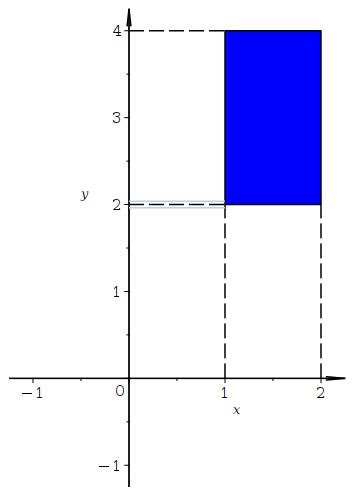
\includegraphics[width=0.25\paperwidth]{example.2.1}

Тепер застосуємо теорему про зведення кратного інтегралу до повторного:
\[
\iint\limits_{D}\left(x^2+y^2\right)d x d y = \int\limits_1^2\left(\int\limits_{2}^{4}\left(x^{2}+y^{2}\right)d y\right)dx.
\]
\begin{remark}
Можна було використати інший порядок змінних $x$ і $y$ і отримати
\[
\iint\limits_{D}\left(x^2+y^2\right)d x d y = \int\limits_{2}^{4}\left(\int\limits_1^2\left(x^{2}+y^{2}\right) d x\right)d y.
\]
В якості вправи пропонуємо підрахувати цей повторний інтеграл і переконатись, що відповідь буде така сама.
\end{remark}
Знайдемо спочатку $\int\limits_{2}^{4}\left(x^{2}+y^{2}\right)d y$. Нагадаємо властивість лінійності інтеграла Рімана:
\[
\int\limits_{a}^{b}\left(f(y)+g(y)\right)d y = \int\limits_{a}^{b}f(y)d y+\int\limits_{a}^{b}g(y)d y.
\]
Тут
\[
\begin{array}{cc}
f(y) = x^2 & \mbox{ --- не залежить від } y\mbox{, при інтегруванні вважається константою!}\\
g(y) = y^2 &
\end{array}
\]
\[
\int\limits_{2}^{4}\left(x^{2}+y^{2}\right)d y = \int\limits_{2}^{4}x^{2}d y+\int\limits_{2}^{4}y^{2}d y
\]

Для знаходження першого доданку ${\int\limits_{2}^{4}x^{2}d y}$ спочатку знайдемо первісну функції ${x^2}$ (яка не залежить від змінної $y$, тобто є в цьому інтегралі константою!):
\[
\int x^{2}d y = x^2 y + C,
\]
а потім скористаємось формулою Ньютона--Лейбніця:
\[
\int\limits_{2}^{4}x^{2}d y = x^2 y \biggr|_{y=2}^4 = 4 x^2 - 2 x^2 = 2 x^2.
\]
Для знаходження другого доданку ${\int\limits_{2}^{4}y^{2}d y}$ спочатку знайдемо первісну функції ${y^2}$:
\[
\int\limits_{2}^{4}y^{2}d y = \frac{y^3}{3} + C,
\]
а потім скористаємось формулою Ньютона--Лейбніця:
\[
\int\limits_{2}^{4}y^{2}d y = \frac{y^3}{3} \biggr|_{y=2}^4 = \frac{4^3}{3} - \frac{2^3}{3} = \frac{56}{3}.
\]
У підсумку,
\[
\int\limits_{2}^{4}\left(x^{2}+y^{2}\right)d y = \int\limits_{2}^{4}x^{2}d y+\int\limits_{2}^{4}y^{2}d y = 2 x^2 + \frac{56}{3}.
\]
Значить,
\[
\iint\limits_{D}\left(x^2+y^2\right)d x d y = \int\limits_1^2\left(\int\limits_{2}^{4}\left(x^{2}+y^{2}\right)d y\right)dx = \int\limits_1^2\left(2 x^2 + \frac{56}{3}\right)dx.
\]
Знайдемо останній інтеграл. Згідно з лінійністю інтеграла Рімана
\[
\int\limits_1^2\left(2 x^2 + \frac{56}{3}\right)dx = 2 \int\limits_1^2 x^2 d x + \frac{56}{3}\int\limits_1^2dx.
\]
Для знаходження першого доданку ${2\int\limits_1^2 x^2 d x}$ спочатку знайдемо первісну функції ${x^2}$ (тепер ми інтегруємо по змінній $x$, і тому ця функція не  є в цьому інтегралі константою):
\[
\int x^{2}d x = \frac{x^3}{3} + C,
\]
а потім скористаємось формулою Ньютона--Лейбніця:
\[
2\int\limits_{1}^{2}x^{2}d x = 2 \times\frac{x^3}{3} \biggr|_{1}^2 = 2\times \frac{2^3}{3} - 2\times \frac{1^3}{3} = \frac{14}{3}.
\]
Для знаходження другого доданку ${\frac{56}{3}\int\limits_1^2dx}$ спочатку знайдемо первісну константи ${1}$:
\[
\int\limits d x = x + C,
\]
а потім скористаємось формулою Ньютона--Лейбніця:
\[
\frac{56}{3}\int\limits_{1}^{2} d x = \frac{56}{3} x \biggr|_{1}^2 = \frac{56}{3}\times 2 - \frac{56}{3} \times 1 = \frac{56}{3}.
\]
У підсумку,
\[
\iint\limits_{D}\left(x^2+y^2\right)d x d y =  \int\limits_1^2\left(2 x^2 + \frac{56}{3}\right)dx = .\frac{14}{3} + \frac{56}{3} = \frac{70}{3}.
\]
Відповідь: ${\iint\limits_{D}\left(x^2+y^2\right)d x d y = .\frac{14}{3} + \frac{56}{3} = \frac{70}{3}.}$
\end{example}

\begin{example}
Знайти ${\iint\limits_{D}8 x^2 \sin\left(4 x y\right)d x d y}$, де через $D$ позначений пря\-мо\-кут\-ник ${D = \segment{\frac{\pi}{2}}{\pi}\times\segment{0}{1}}$.

Спочатку зробимо рисунок області інтегрування $D$.

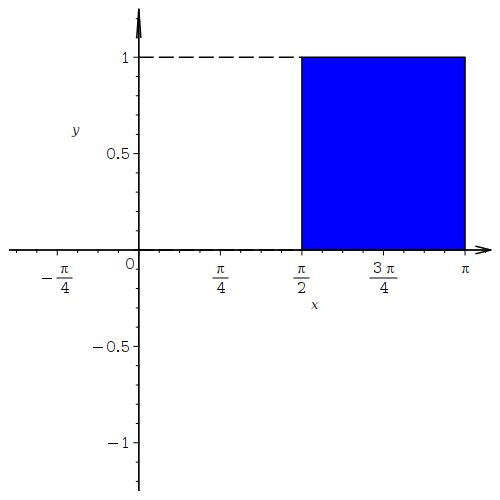
\includegraphics[width=0.25\paperwidth]{example.2.2}

Тепер застосуємо теорему про зведення кратного інтегралу до повторного:
\[
\iint\limits_{D}8 x^2 \sin(4 x y)d x d y = \int\limits_{\frac{\pi}{2}}^{\pi}\left(\int\limits_{0}^{1}8 x^2 \sin\left(4 x y\right)d y\right)dx.
\]

Знайдемо спочатку $\int\limits_{0}^{1}8 x^2 \sin\left(4 x y\right)d y$. Нагадаємо властивість лінійності інтеграла Рімана:
\[
\int\limits_{a}^{b}\alpha f(y) d y = \alpha \int\limits_{a}^{b}f(y)d y.
\]
Тут
\[
\begin{array}{cc}
f(y) =  \sin\left(4 x y\right) & \\
\alpha = 8 x^2  & \mbox{ --- не залежить від } y\mbox{, при інтегруванні вважається константою!}
\end{array}
\]
\[
\int\limits_{0}^{1}8 x^2 \sin\left(4 x y\right)d y = 8 x^2 \int\limits_{0}^{1} \sin\left(4 x y\right)d y.
\]
Тепер знайдемо первісну функції ${\sin\left(4 x y\right)}$:
\[
\int\limits \sin\left(4 x y\right)d y = -\frac{1}{4 x}\cos\left(4 x y\right) + C,
\]

а потім скористаємось формулою Ньютона--Лейбніця:
\[
\int\limits_{0}^1 \sin\left(4 x y\right)d y = -\frac{1}{4 x}\cos\left(4 x y\right) \biggr|_{y=0}^1 = -\frac{1}{4 x}\cos\left(4 x\right) - \left(-\frac{1}{4 x}\cos\left(0\right)\right) = \frac{1 - \cos \left(4 x\right)}{4 x}.
\]
У підсумку,
\[
\int\limits_{0}^{1}8 x^2 \sin\left(4 x y\right)d y = 8 x^2\times \frac{1 - \cos \left(4 x\right)}{4 x} = 2x \left(1 - \cos \left(4 x\right)\right).
\]
Значить,
\[
\iint\limits_{D}8 x^2 \sin(4 x y)d x d y = \int\limits_{\frac{\pi}{2}}^{\pi} 2x \left(1 - \cos \left(4 x\right)\right) d x.
\]
Знайдемо останній інтеграл. Для знаходження визначеного інтегралу
\[
\int\limits_{\frac{\pi}{2}}^{\pi} 2x \left(1 - \cos \left(4 x\right)\right) d x
\]
потрібно скористатись формулою інтегрування частинами:
\[
\int_a^b u d v = u v\biggr|_a^b - \int_a^b v d u.
\]
Тут
\[
\begin{array}{l}
u = 2 x, \\
d v = \left(1 - \cos \left(4 x\right)\right) d x.
\end{array}
\]
Для знаходження ${d u}$ потрібно продифференціювати (знайти похідну) ${u}$:
\[
d u  = \left(2 x \right)' d x = 2 d x,
\]
a для знаходження $v$ потрібно проінтегрувати ${d v}$:
\[
v = \int \left(1 - \cos \left(4 x\right)\right) d x \stackrel{{\normalfont\mbox{\tiny{(лінійність!})}}}{=} \int d x - \int \cos\left(4 x\right) d x = x - \frac{1}{4}\sin\left(4 x\right) + C.
\]
Таким чином,
\[
\begin{array}{l}
\int\limits_{\frac{\pi}{2}}^{\pi} 2x \left(1 - \cos \left(4 x\right)\right) d x = \left(2 x \left(x - \frac{1}{4}\sin\left(4 x\right)\right)\right)\biggr|_\frac{\pi}{2}^\pi - \int\limits_{\frac{\pi}{2}}^{\pi} \left(x - \frac{1}{4}\sin\left(4 x\right)\right) 2 d x = \\ =
\left(2 \pi \left(\pi - \frac{1}{4}\sin\left(4 \pi\right)\right)\right) - \left(2 \frac{\pi}{2} \left(\frac{\pi}{2} - \frac{1}{4}\sin\left(4\times \frac{\pi}{2}\right)\right)\right) - \int\limits_{\frac{\pi}{2}}^{\pi} \left(2x - \frac{1}{2}\sin\left(4 x\right)\right) d x = \\
=2\pi^2 - \frac{\pi^2}{2} - \int\limits_{\frac{\pi}{2}}^{\pi} \left(2x - \frac{1}{2}\sin\left(4 x\right)\right) d x = \frac{3\pi^2}{2} - \int\limits_{\frac{\pi}{2}}^{\pi} \left(2 x - \frac{1}{2}\sin\left(4 x\right)\right) d x.
\end{array}
\]
Для знаходження інтегралу ${\int\limits_{\frac{\pi}{2}}^{\pi} \left(2 x - \frac{1}{2}\sin\left(4 x\right)\right) d x}$ спочатку скористаємось лінійністю
\[
\int\limits_{\frac{\pi}{2}}^{\pi} \left(2 x - \frac{1}{2}\sin\left(4 x\right)\right) d x = 2\int\limits_{\frac{\pi}{2}}^{\pi} x d x - \frac{1}{2} \int\limits_{\frac{\pi}{2}}^{\pi} \sin\left(4 x\right) d x,
\]
потім знайдемо первісні функцій $x$ і $\sin\left(4 x\right)$
\[
\begin{array}{c}
\int x d x = \frac{x^2}{2} + C,\\
\int \sin\left(4 x\right) d x = -\frac{1}{4}\cos\left(4 x\right) + C,
\end{array}
\]
а потім скористаємось формулою Ньютона--Лейбніця:
\[
\begin{array}{c}
\int\limits_{\frac{\pi}{2}}^{\pi} x d x = \frac{x^2}{2}\biggr|_\frac{\pi}{2}^\pi = \frac{\pi^2}{2} - \frac{(\frac{\pi}{2})^2}{2} = \frac{\pi^2}{2} - \frac{\pi^2}{8} = \frac{3\pi^2}{8},\\
\int\limits_{\frac{\pi}{2}}^{\pi} \sin\left(4 x\right) d x = -\frac{1}{4}\cos\left(4 x\right)\biggr|_\frac{\pi}{2}^\pi = -\frac{1}{4}\cos\left(4 \pi\right) - \left(-\frac{1}{4}\cos\left(4 \times \frac{\pi}{2}\right)\right) = 0.
\end{array}
\]
У підсумку,
\[
\int\limits_{\frac{\pi}{2}}^{\pi} \left(2 x - \frac{1}{2}\sin\left(4 x\right)\right) d x = 2\int\limits_{\frac{\pi}{2}}^{\pi} x d x - \frac{1}{2} \int\limits_{\frac{\pi}{2}}^{\pi} \sin\left(4 x\right) d x = 2\times \frac{3\pi^2}{8} - \frac{1}{2} \times 0 = \frac{3\pi^2}{4},
\]
значить,
\[
\int\limits_{\frac{\pi}{2}}^{\pi} 2x \left(1 - \cos \left(4 x\right)\right) d x = \frac{3\pi^2}{2} - \frac{3\pi^2}{4} = \frac{3\pi^2}{4}.
\]
Остаточно,
\[
\iint\limits_{D}8 x^2 \sin(4 x y)d x d y = \frac{3\pi^2}{4}.
\]
Відповідь: ${\iint\limits_{D}8 x^2 \sin(4 x y)d x d y = \frac{3\pi^2}{4}.}$
\begin{remark}
В цьому прикладі ми також могли використати інший порядок змінних при зведенні до повторного інтегралу, і ми б отримали наступну рівність:
\[
\iint\limits_{D}8 x^2 \sin(4 x y)d x d y = \int\limits_{0}^{1}\left(\int\limits_{\frac{\pi}{2}}^{\pi}8 x^2 \sin\left(4 x y\right)d x\right)dy.
\]
Але в цьому випадку знаходження інтегралу всередині буде відносно складним і в результаті ми отримаємо
\[
\begin{array}{c}
\int\limits_{\frac{\pi}{2}}^{\pi}8 x^2 \sin\left(4 x y\right)d x = \\= -\dfrac{8 \pi^{2} y^{2} \cos \! \left(4 y \pi \right)-2 y^{2} \cos \! \left(2 y \pi \right) \pi^{2}-4 y \pi  \sin \! \left(4 y \pi \right)}{4 y^{3}}+\\
+\dfrac{2 y \sin \! \left(2 y \pi \right) \pi -\cos \! \left(4 y \pi \right)+\cos \! \left(2 y \pi \right)}{4 y^{3}}.
\end{array}
\]
Останній вираз потрібно буде ще проінтегрувати по $y$ від~$0$~до~$1$, що буде значно складніше наведеного розв'язання. Таким чином,

\fbox{
\begin{minipage}{0.7\textwidth}
\textbf{складність знаходження подвійного інтегралу може суттєво залежати від того, в якому порядку зводити його до повторного.}
\end{minipage}
}
\end{remark}
\end{example}
\begin{example}
Знайти ${\iiint\limits_{V}\left(x + y^2 - 2 z\right)d x d y d z}$, де через $V$ позначений пря\-мо\-кут\-ний паралелепіпед ${V = \segment{1}{2}\times\segment{1}{3}\times\segment{4}{5}}$.
Застосуємо теорему про зведення кратного інтегралу до повторного:
\[
\iiint\limits_{V}\left(x + y^2 - 2 z\right)d x d y d z = \int\limits_1^2\left(\int\limits_1^3\left(\int\limits_4^5\left(x + y^2 - 2 z\right)d z\right)d y\right)d x.
\]

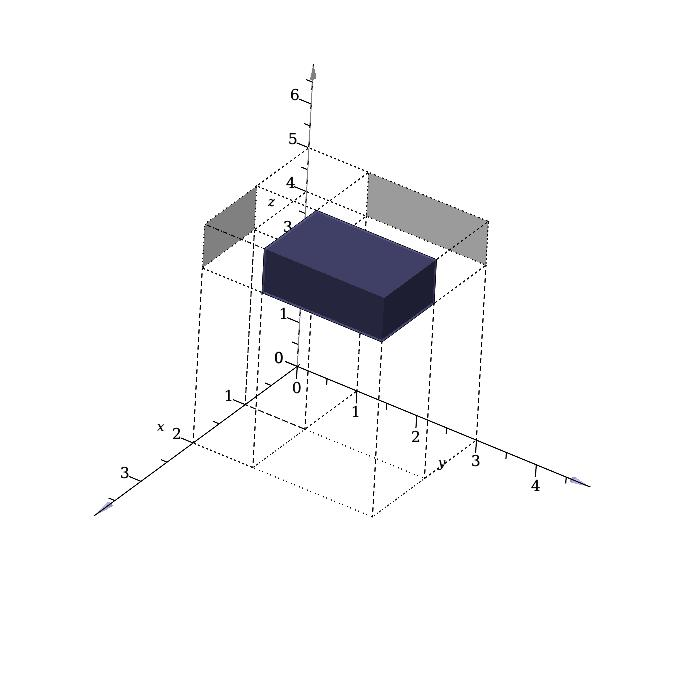
\includegraphics[width=0.5\paperwidth]{example.2.3}

Знайдемо спочатку ${\int\limits_4^5\left(x + y^2 - 2 z\right)d z}$. З лінійності інтеграла Рімана випливає, що
\[
\int\limits_4^5\left(x + y^2 - 2 z\right)d z = \int\limits_4^5xd z + \int\limits_4^5y^2d z - 2 \int\limits_4^5 zd z.
\]
Тепер знайдемо первісні відповідних функцій (пам'таємо, що інтегрування відбувається по змінній $z$, тому змінні $x$ та $y$ при цьому є константами):
\[
\begin{array}{c}
\int x d z = x z + C,\\
\int y^2 d z = y^2 z + C,\\
\int z d z = \frac{z^2}{2} + C,
\end{array}
\]

а потім скористаємось формулою Ньютона--Лейбніця:
\[
\begin{array}{c}
\int\limits_4^5 x d z = x z\biggr|_{z=4}^5 = 5 x - 4 x = x,\\
\int\limits_4^5 y^2 d z = y^2 z\biggr|_{z=4}^5 = 5 y^2 -4 y^2 = y^2,\\
\int\limits_4^5 z d z = \frac{z^2}{2}\biggr|_{z=4}^5 = \frac{25}{2} - \frac{16}{2} = \frac{9}{2},
\end{array}
\]
Таким чином,
\[
\int\limits_4^5\left(x + y^2 - 2 z\right)d z = x + y^2 - 2 \times .\frac{9}{2} = x + y^2 -9
\]
і
\[
\iiint\limits_{V}\left(x + y^2 - 2 z\right)d x d y d z = \int\limits_1^2\left(\int\limits_1^3\left(x + y^2 -9\right)d y\right)d x.
\]
Тепер шукаємо
\[
\int\limits_1^3\left(x + y^2 -9\right)d y \stackrel{{\normalfont\mbox{(лінійність)}}}{=} \int\limits_1^3 x d y  + \int\limits_1^3 y^2d y  - 9 \int\limits_1^3 d y.
\]
Тепер знайдемо первісні відповідних функцій (пам'таємо, що інтегрування відбувається по змінній $y$, тому змінна $x$ при цьому є константою):
\[
\begin{array}{c}
\int x d y = x y + C,\\
\int y^2 d y = \frac{y^3}{3} + C,\\
\int d y = y + C,
\end{array}
\]

а потім скористаємось формулою Ньютона--Лейбніця:
\[
\begin{array}{c}
\int\limits_1^3 x d y = x y\biggr|_{y=1}^3 = 3 x - x = 2 x,\\
\int\limits_1^3 y^2 d y = \frac{y^3}{3}\biggr|_{y=1}^3 = \frac{3^3}{3} - \frac{1^3}{3} = \frac{26}{3},\\
\int\limits_1^3 d y = y\biggr|_{y=1}^3 = 3 - 1 = 2.
\end{array}
\]
Далі
\[
\int\limits_1^3\left(x + y^2 -9\right)d y = 2 x  +\frac{26}{3} - 9 \times 2 = 2 x - \frac{28}{3}.
\]
і
\[
\iiint\limits_{V}\left(x + y^2 - 2 z\right)d x d y d z = \int\limits_1^2\left(2 x - \frac{28}{3}\right)d x.
\]
Знайдемо останній інтеграл.
\[
\int\limits_1^2\left(2 x - \frac{28}{3}\right)d x \stackrel{{\normalfont\mbox{(лінійність)}}}{=} 2 \int\limits_1^2 x d x - \frac{28}{3} \int\limits_1^2 d x.
\]
Первісні:
\[
\begin{array}{c}
\int x d x = \frac{x^2}{2} + c,\\
\int d x  = x + C.
\end{array}
\]
Тепер формула Ньютона--Лейбніця:
\[
\begin{array}{c}
\int x d x = \frac{x^2}{2}\biggr|_{1}^2 = \frac{2^2}{1} - \frac{1^2}{2} = \frac{3}{2},\\
\int d x  = x \biggr|_{1}^2 = 2 - 1 = 1,\\
\end{array}
\]
Остаточно,
\[
\iiint\limits_{V}\left(x + y^2 - 2 z\right)d x d y d z = 2 \times \frac{3}{2}- \frac{28}{3} \times 1 = -\frac{19}{3}.
\]
Відповідь: ${-\frac{19}{3}}$.
\end{example}
\nocite{Gar84}


\part{Вимірні множини}\label{part:measure}
Наша наступна мета --- визначити кратні інтеграли не тільки по гіперпрямокутниках, а і по множинах більш широкого класу. Цей клас --- клас вимірних за Жорданом множин. До визначення цього класу ми зараз і переходимо.
\section{Розбиття простору \eucl{m}}
\begin{definition}
Розбиттям нульового порядку простору \eucl{m} будемо називати зображення простору \eucl{m} у вигляді об'єднання всіх можливих брусів. сторони яких є відрізками довижини 1 з цілими координатами:
\[
\eucl{m} = \bigcup\limits_{n_1, n_2, \ldots, n_m\in\Z}\segment{n_1}{n_1+1}\times\segment{n_2}{n_2+1}\times\ldots\times\segment{n_m}{n_m+1}.
\]
\end{definition}
\begin{definition}
Розбиттям $k$--го порядку для ${k\in\N}$ простору \eucl{m} будемо називати зображення простору \eucl{m} у вигляді об'єднання всіх можливих брусів, сторони яких є відрізками довижини ${\frac{1}{2^k}}$ з координатами, які можуть бути надані у вигляді раціонального дробу (можливо, скоротного) ${\frac{n}{2^k}}$, ${n\in\Z}$:
\[
\eucl{m} = \bigcup\limits_{n_1, n_2, \ldots, n_m\in\Z}\segment{\frac{n_1}{2^k}}{\frac{n_1+1}{2^k}}\times\segment{\frac{n_2}{2^k}}{\frac{n_2+1}{2^k}}\times\ldots\times\segment{\frac{n_m}{2^k}}{\frac{n_m+1}{2^k}}.
\]
\end{definition}
Множину всіх брусів розбиття порядку $k$, ${k\in\N\cup\{0\}}$ будемо позначати ${\pi^{(k)}}$:
\[
\pi^{(k)} =
\left\{
\left.
\segment{\frac{n_1}{2^k}}{\frac{n_1+1}{2^k}}\times\segment{\frac{n_2}{2^k}}{\frac{n_2+1}{2^k}}\times\ldots\times\segment{\frac{n_m}{2^k}}{\frac{n_m+1}{2^k}}
\right| n_1, n_2, \ldots, n_m\in\Z
\right\}.
\]
\section{Міра Жордана}
\hyperref[def:box]{Нагадаємо}, що мірою брусу
\[
Q = \segment{a_1}{b_1}\times\segment{a_2}{b_2}\times\ldots\times\segment{a_m}{b_m} \subset \eucl{m},
\]
називають число
\[
\m(Q) = \left(b_1-a_1\right)\left(b_2 - a_2\right)\ldots\left(b_m-a_m\right) = \prod\limits_{j=1}^{m}\left(b_j - a_j\right).
\]
\begin{definition}
Якщо множина ${A\subset\eucl{m}}$ є об'єднанням скінченої кількості брусів, внутрішності яких попарно не перетинаються,
\[
A = \bigcup\limits_{j=1}^nQ_j,
\]
то мірою $A$ будемо називати суму мір цих брусів:
\[
\m\left(A\right) = \sum\limits_{j=1}^n\m\left(Q_j\right).
\]
Зокрема, мірою порожньої множини будемо вважати 0:
\[
\m(\emptyset) = 0.
\]
\end{definition}
Це означення, зокрема, можна застосовувати для тих випадків, коли ${Q_1}$, ${Q_2}$, ${\ldots}$, ${Q_n}$ --- різні бруси певного розбиття ${\pi^{(k)}}$.

Нехай тепер ${A\subset\eucl{m}}$ --- довільна обмежена множина, ${\pi^{(k)}}$ --- розбиття \eucl{m}, $k\in\N\cup\{0\}$. Введемо наступні позначення:
\begin{itemize}\label{partition_sets}
\item $A_{(k)}$ --- об'єднання всіх брусів з ${\pi^{(k)}}$, які є підмножиною $A$:
\[
A_{(k)} = \bigcup\limits_{\tiny{\begin{array}{c}Q\in\pi^{(k)}\\Q\subset A\end{array}}}Q;
\]
\item $A^{(k)}$ --- об'єднання всіх брусів з ${\pi^{(k)}}$, які мають непорожній перетин з $A$:
\[
A_{(k)} = \bigcup\limits_{\tiny{\begin{array}{c}Q\in\pi^{(k)}\\Q\cap A\neq \emptyset\end{array}}}Q;
\]
\item $\Delta A^{(k)}$ --- різниця множин $A^{(k)}$ і $A_{(k)}$:
\[
\Delta A_{(k)} = A^{(k)} \setminus A_{(k)}.
\]
\end{itemize}
У випадках, коли описаних вище брусів не існує, будемо вважати відповідну множину порожньою.
Множини ${A_{(k)}}$, ${A^{(k)}}$ і ${\Delta A_{(k)}}$ мають наступні властивості:
\begin{itemize}
\item ${A_{(k)} \subset A \subset A^{(k)}}$,
\item ${A_{(k)} \subset A_{(k+1)}}$,
\item ${A^{(k+1)} \subset A^{(k)}}$.
\end{itemize}
Оскільки всі три множини ${A_{(k)}}$, ${A^{(k)}}$ і ${\Delta A_{(k)}}$ є об'єднаннями брусів розбиття ${\pi^{(k)}}$, то визначені їх міри ${\m\left(A_{(k)}\right)}$, ${\m\left(A^{(k)}\right)}$ і ${\m\left(\Delta A_{(k)}\right)}$, причому зозначення і властивостей множин випливають властивості їх мір:
\begin{itemize}
\item ${0 \leq \m\left(A_{(k)}\right) \leq \m\left(A^{(k)}\right)}$,
\item ${\m\left(A_{(k)}\right) \leq \m\left(A_{(k+1)}\right)}$,
\item ${\m\left(A^{(k+1)}\right) \leq \m\left(A^{(k)}\right)}$,
\item ${\m\left(\Delta A_{(k)}\right) = \m\left(A^{(k)}\right) - \m\left(A_{(k)}\right)}$.
\end{itemize}
З цих властивостей, зокрема, випливає, що обидві послідовності ${\left\{\m\left(A_{(k)}\right)\right\}}$ і ${\left\{\m\left(A^{(k)}\right)\right\}}$ є обмеженими і монотонними, а значить, збіжними.
\begin{definition}
Внутрішньою мірою обмеженої множини ${A\subset\eucl{m}}$ будемо називати число
\[
\m_{*}\left(A\right) = \lim\limits_{k\to\infty}\m\left(A_{(k)}\right).
\]
Зовнішньою мірою множини ${A}$ будемо називати число
\[
\m^{*}\left(A\right) = \lim\limits_{k\to\infty}\m\left(A^{(k)}\right).
\]
\end{definition}
З властивостей міри множин ${A_{(k)}}$ і ${A^{(k)}}$ випливає, що
\[
0 \leq \m_{*}\left(A\right) \leq \m^{*}\left(A\right)
\]
для довільної обмеженої множини $A$.
\begin{definition}
Обмежену множину ${A\subset\eucl{m}}$ будемо називати вимірною за Жорданом, якщо
\[
\m_{*}\left(a\right) = \m^{*}\left(a\right).
\]
В цьому випадку спільне значення ${\m_{*}\left(a\right) = \m^{*}\left(a\right)}$ будемо називати ($m$--вимірною) мірою Жордана множини $A$ і будемо позначати ${\m\left(A\right)}$:
\[
\m\left(A\right) =\m_{*}\left(A\right) = \m^{*}\left(A\right).
\]
\end{definition}
Вимірні за Жорданом множини мають наступні властивості:
\begin{itemize}
\item\label{prop:measrable_sets:1} якщо $A$ і $B$ --- вимірні за Жорданом, то і ${A\cup B}$ також є вимірною за Жорданом;
\item якщо $A$ і $B$ --- вимірні за Жорданом, то і ${A\cap B}$ також є вимірною за Жорданом;
\item якщо $A$ і $B$ --- вимірні за Жорданом, то і ${A\setminus B}$ також є вимірною за Жорданом.
\end{itemize}
Міра Жордана має наступні властивості:
\begin{enumerate}
\item ${\m\left(A\right)\geq 0}$ для довільної вимрної за Жорданом множини ${A}$;
\item {\bf напівадидивність}:
${\m\left(A\cup B\right) \leq \m\left(A\right) + \m\left(B\right)}$ для довільних вимрних за Жорданом множин ${A}$ і ${B}$;
\item {\bf адидивність}:
${\m\left(A\cup B\right) = \m\left(A\right) + \m\left(B\right)}$ для довільних вимрних за Жорданом множин ${A}$ і ${B}$, внутрішності яких не перетинаються;
\item {\bf монотонність}: ${\m\left(A\right)\leq \m\left(B\right)}$ для довільних вимрних за Жорданом множин ${A\subset B}$.
\end{enumerate}
Важливим класом вимвірних множин є циліндричні множини, визначені в наступному означенні.
\begin{definition}
Нехай ${m\geq2}$. У просторі \eucl{m-1} розглянемо множину ${A \subset \eucl{m-1}}$ і дві функції
\[
u_1,u_2\colon A\to \R,
\]
які задовольняють наступну властивість:
\[
\forall \left(x_1, x_2, \ldots, x_{m-1}\right)\in A\ u_1\left(x_1, x_2, \ldots, x_{m-1}\right)\leq u_2\left(x_1, x_2, \ldots, x_{m-1}\right).
\]
Тоді множину
\[
C =
\left\{
\left(x_1, x_2, \ldots, x_{m-1}, x_m\right)
\left|
\begin{array}{c}
\left(x_1, x_2, \ldots, x_{m-1}\right)\in A,\\
u_1\left(x_1, x_2, \ldots, x_{m-1}\right)\leq x_m \leq u_2\left(x_1, x_2, \ldots, x_{m-1}\right)
\end{array}
\right.
\right\}
\]
будемо називати циліндричною в напрямку осі ${Ox_m}$ з основою $A$. Основу циліндричної множини $C$ будемо позначати ${\ba C}$:
\[
A = \ba C.
\]
\end{definition}
Вимірність широкого класу циліндричних множин встановлюється наступною теоремою.
\begin{theorem}
Нехай $C$ --- циліндрична множина, що визначається основою $\ba C$ і функціями ${u_1, u_2\colon \ba C\to \R.}$ Якщо
\begin{enumerate}
\item $\ba C$ --- компактна вимірна підмножина \eucl{m-1},
\item функції $u_1$ і $u_2$ неперервні на $\ba C$,
\end{enumerate}
то множина $C$ --- компактна і вимірна.
\end{theorem}

\part{Кратні інтеграли по вимірних множинах}
\section{Означення}
Нагадаємо, що кратні інтеграли по брусах були визначені в розділі~\ref{part:boxes}. Тепер в два кроки ми поширемо клас множин, по яких визначаються кратні інтеграли, від брусів до вимірних множин.
\begin{definition}
Нехай множина ${A\subset\eucl{m}}$ є об'єднанням скінченої кількості брусів
\[
A = \bigcup\limits_{j=1}^nQ_j,
\]
внутрішності яких попарно не перетинаються  (бруси ${Q_j}$ і ${Q_k }$ не мають спільних внутрішнії точок при ${j\neq k}$), а функція ${f\colon A\to \R}$ неперервна на $A$. Інтеграл від функції $f$ по множині $A$ визначимо наступною формулою
\[
\int\limits_Af(x) d x = \sum\limits_{j=1}^n\int\limits_{Q_j}f(x) d x.
\]
\end{definition}
\begin{remark}
Зауважимо, що останнє означення може бути застосоване для множин ${A_{(k)}}$, де $A$ --- довільна обмежена множина (дивись \hyperref[partition_sets]{позначення} в розділі~\ref{part:measure}).
\end{remark}
Виявляється, що має місце наступна лема.
\begin{lemma}
Нехай ${A\subset\eucl{m}}$ --- вимірна множина, а функція ${f\colon A\to\R}$ --- неперервна і обмежена на ${A}$. Тоді послідовність ${\left\{\int\limits_{A_{(k)}}f(x) d x\right\}_{k=1}^\infty}$ є фундаментальною (а значить, збіжною!).
\end{lemma}
Ця лема дає можливість визначити кратні інтеграли по вимірних множинах.
\begin{definition}
Нехай ${A\subset\eucl{m}}$ --- вимірна множина, а функція ${f\colon A\to\R}$ --- неперервна і обмежена на ${A}$. Число
\[
\int\limits_{A}f(x) d x = \lim\limits_{k\to\infty}\int\limits_{A_{(k)}}f(x) d x
\]
будемо називати ${m}$--кратним інтегралом від функції  по множині ${A}$. Якщо ${\m\left(A\right) = 0}$, то ${A_{(k)} = \emptyset}$ для всіх ${k\in\N}$, тому в цьому випадку природньо поклдасти за означенням ${\int\limits_{A}f(x) d x = 0}$.
\end{definition}

Властивості кратних інтегралів по вимірних множинах аналогічні властивостям кроатних інтегралів по гіперпрямокутникам.
\begin{enumerate}
\item Інтеграл від константи.
\begin{intextProposition}
Для довільної дійсної константи $c$ стала функція ${f(x) \equiv c}$ інтегровна на довільній вимірниій множині $A$, причому
\[
\int\limits_{A} c d x = c\m\left(Q\right).
\]
\end{intextProposition}
\item Лінійність
\begin{intextProposition}
Якщо обидві функції ${f\colon A \to \R}$ і ${g\colon Q \to \R}$ неперервні і обмежені на вимірній множині $A$, то для довільних дійсних чисел $\alpha$ і $\beta$ виконується рівність
\[
\int\limits_{A} \left(\alpha f(x) + \beta g(x)\right)d x = \alpha\int\limits_{A} f(x) d x + \beta\int\limits_{A} g(x) d x.
\]
\end{intextProposition}
\item Аддитивність
\begin{intextProposition}
Якщо множина $A$ є об'єднанням двох вимірних множин --- ${A = A_1 \cup A_2}$, причому вимірні множини $A_1$ і $A_2$ не мають спільних внутрішніх точок, а функція ${f\colon A \to \R}$ неперервна і обмежена на $A$, то
\[
\int\limits_{A} f(x) d x = \int\limits_{A_1} f(x) d x + \int\limits_{A_2} f(x) d x.
\]
\end{intextProposition}
\begin{remark}
Окільки $A_1$ і $A_2$ --- вимірні множини, то і ${A = A_1 \cup A_2}$ --- вимірна множина за \hyperref[prop:measrable_sets:1]{властивістю вимірних множин}.
\end{remark}
\item Невід'ємність
\begin{intextProposition}
Якщо функція ${f\colon A \to \R}$ неперервна і обмежена на вимірній множині $A$ і ${\forall x\in A\ f(x)\geq 0}$, то ${\int\limits_{A} f(x) d x \geq 0.}$
\end{intextProposition}
\item Монотонність
\begin{intextProposition}
Якщо обидві функції ${f\colon A \to \R}$ і ${g\colon A \to \R}$ неперервні і обмежені на вимірній множині $A$ і ${\forall x\in A\ f(x)\geq g(x)}$, то ${\int\limits_{A} f(x) d x \geq \int\limits_{A} g(x) d x.}$
\end{intextProposition}
\item Модуль інтеграла
\begin{intextProposition}
Якщо функція ${f\colon A \to \R}$ неперервна і обмежена на вимірній множині $A$, то
\[
\left|\int\limits_{A} f(x) d x\right| \leq \int\limits_{A} \left|f(x)\right| d x.
\]
\end{intextProposition}
\end{enumerate}
\begin{remark}
Формулювання теореми про середнє значення у випадку кратних інтегралів по вимірних множинах потребує поняття лінійної зв'язності множин, і тому ми його тут не приводимо.
\end{remark}

Обчислення кратних інтегралів відбувається шляхом зведення них до повторних на підставі наступної теореми.
\begin{theorem}
Нехай задані циліндрична множина $C$, що визначається основою $\ba C$ і функціями ${u_1, u_2\colon \ba C\to \R}$ і функція $f\colon C\to \R$. Якщо
\begin{enumerate}
\item $\ba C$ --- компактна вимірна підмножина \eucl{m-1},
\item функції $u_1$ і $u_2$ неперервні на $\ba C$,
\item функція $f$ неперервна на $C$.
\end{enumerate}
Тоді має місце наступна рівність:
\[
\begin{array}{c}
\int\limits_C f(x)d x = \\
 =\int\limits_{\ba C}\left( \int\limits_{u_1\left(x_1, x_2,\ldots, x_{m-1}\right)}^{u_2\left(x_1, x_2,\ldots, x_{m-1}\right)} f\left(x_1, \ldots, x_{m-1}, x_m \right)d x_m\right) d x_1 \ldots  d x_{m-1}.
\end{array}
\]
\end{theorem}
\section{Приклади обчислень}
\begin{example}
Знайти ${\iint\limits_D y^3 x^2 d x d y}$, де через $D$ позначена область на площині обмежена лініями ${x = 0}$, ${y = x}$, ${x + y = 2}$.

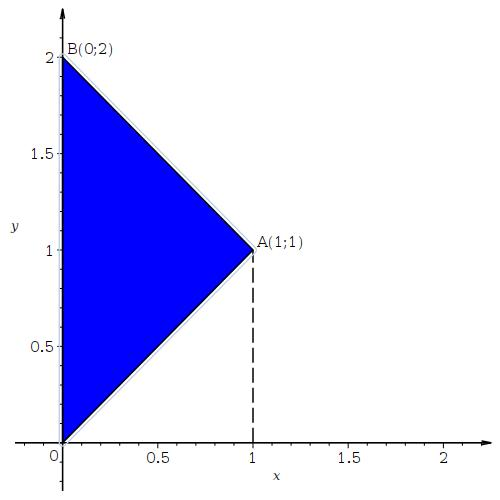
\includegraphics[width=0.5\paperwidth]{example.2.4}

Область $D$ є множиною на площині циліндричною в напрямку осі ${Oy}$, що визначається основою ${\left[0;1\right]}$. Для того, щоб знайти функції ${u_1, u_2\colon \left[0;1\right]\to \R}$, що визначають циліндричну множину $D$, потрібно записати рівняння ліній ${OA}$ і ${AB}$ --- ${y = x}$ і ${x + y =2 }$ відповідно, і виразити з них $y$ через $x$. Отримаємо
\[
\begin{array}{l}
u_1(x) = x,\\ u_2(x) = 2 - x.
\end{array}
\]
Згідно з теоремою про зведення кратного інтегралу до повторного маємо
\[
\iint\limits_D y^3 x^2 d x d y = \int\limits_0^1 \int\limits_{x}^{2 - x} y^3 x^2 d y d x.
\]
Спочатку знайдемо ${\int\limits_{x}^{2 - x} y^3 x^2 d y}$. З лiнiйностi iнтеграла Рiмана випливає, що
\[
\int\limits_{x}^{2 - x} y^3 x^2 d y = x^2 \int\limits_{x}^{2 - x} y^3  d y
\]
(пам’таємо, що iнтегрування вiдбувається по змiннiй $y$, тому змiнна $x$ при цьому є константою).

Тепер знайдемо первiсну:
\[
\int y^3  d y = \frac{y^4}{4} + C.
\]
Згідно з формулою Ньютона-–Лейбнiця:
\[
\int\limits_{x}^{2 - x} y^3 d y = \frac{y^4}{4}\biggr|_{y=x}^{2-x} = \frac{\left(2 - x\right)^4}{4} - \frac{x^4}{4}.
\]
Спростимо останній вираз:
\[
\begin{array}{c}
\dfrac{\left(2 - x\right)^4}{4} - \dfrac{x^4}{4} = \dfrac{2^4 - 4\cdot 2^3\cdot x^3 + 6\cdot 2^2\cdot x^2 - 4 \cdot 2\cdot x + x^4 - x^4}{4} =\\\\=\dfrac{16 - 32 x + 24 x^2 - 8 x^3}{4}  = 4 - 8 x + 6 x^2 -  2 x^3.
\end{array}
\]
Значить,
\[
\int\limits_{x}^{2 - x} y^3 x^2 d y = x^2 \int\limits_{x}^{2 - x} y^3  d y = x^2\left(4 - 8 x + 6 x^2 -  2 x^3\right) = 4 x^2 - 8 x^3 + 6 x^4 -  2 x^5,
\]
і
\[
\iint\limits_D y^3 x^2 d x d y = \int\limits_0^1 \left(4 x^2 - 8 x^3 + 6 x^4 -  2 x^5\right) d x.
\]
Знайдемо останній інтеграл.
\[
\begin{array}{c}
\int\limits_0^1 \left(4 x^2 - 8 x^3 + 6 x^4 -  2 x^5\right) d x =\\
\mbox{(лінійність)} \\
= 4 \int\limits_0^1 x^2  d x - 8 \int\limits_0^1x^3  d x + 6 \int\limits_0^1x^4  d x -  2 \int\limits_0^1x^5 d x  = \\
\mbox{(первісні і формула Ньютона--Лейбнiця)}\\
=4\cdot\dfrac{x^3}{3}\biggr|_0^1 - 8\cdot \dfrac{x^4}{4}\biggr|_0^1 + 6\cdot\dfrac{x^5}{5}\biggr|_0^1 - 2\cdot\dfrac{x^6}{6}\biggr|_0^1 =\\
\mbox{(рахуємо підстановки)}\\
= 4\cdot\dfrac{1^3}{3} - 8\cdot \dfrac{1^4}{4} + 6\cdot\dfrac{1^5}{5} - 2\cdot\dfrac{1^6}{6} - \left(4\cdot\dfrac{0^3}{3} - 8\cdot \dfrac{0^4}{4} + 6\cdot\dfrac{0^5}{5} - 2\cdot\dfrac{0^6}{6}\right) = \\\\
= \dfrac{4}{3} - 2 + \dfrac{6}{5} - \dfrac{1}{3} = \dfrac{1}{5}.
\end{array}
\]

У підсумку,
\[
\iint\limits_D y^3 x^2 d x d y = \dfrac{1}{5}.
\]
\end{example}

\begin{example}
Знайти ${\iint\limits_D \sin y d x d y}$, де через $D$ позначений трикутник на площині з вершинами ${A\left(1;\frac{\pi}{2}\right)}$, ${B\left(2;\frac{\pi}{2}\right)}$, ${C\left(3;\pi\right)}$.

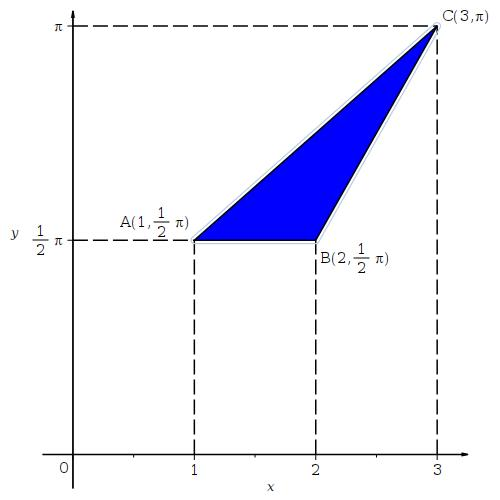
\includegraphics[width=0.5\paperwidth]{example.2.5}

Як і в попередньому прикладі, область $D$ є множиною на площині циліндричною в напрямку осі ${Oy}$. Основою в даному випадку буде відрізок ${\left[1;3\right]}$. Але функція ${u_1(x)}$ в цьому випадку записується двома різними формулами, що відповідають рівнянням прямих ${AB}$ і ${BC}$. Тому цей приклад має сенс ровз'язувати виходячи з того, що множина $D$ є також циліндричною в напрямку осі ${Ox}$. Основою тоді буде відрізок ${\left[\frac{\pi}{2};\pi\right]}$.
\begin{remark}
Якщо все ж таки розглядати множину $D$ як циліндричну в напрямку осі ${Oy}$, то отримаємо наступну рівність
\[
\iint\limits_D \sin y d x d y = \int\limits_{1}^{2}\left(\int\limits_{\frac{\pi}{2}}^{\frac{\pi}{2}+\frac{\pi  \left(x-1\right)}{4}}\sin y dy\right) dx+\int\limits_{2}^{3}\left(\int\limits_{\frac{\pi}{2}+\frac{\pi  \left(x-2\right)}{2}}^{\frac{\pi}{2}+\frac{\pi  \left(x-1\right)}{4}}\sin y dy\right) dx.
\]
Підрахуйте самостійно ці повторні інтеграли і переконайтесь, що відповідь буде така сама.
\end{remark}
Для того, щоб знайти функції ${u_1, u_2\colon \left[\frac{\pi}{2};\pi\right]\to \R}$, що визначають циліндричну множину $D$, потрібно записати рівняння ліній ${AC}$ і ${BC}$ --- ${\frac{\pi}{2}  x+2 y-\frac{\pi}{2} =0}$ і ${\frac{\pi}{2}  x-y-\frac{\pi}{2} =0}$ відповідно, але тепер виразити з них $x$ через $y$. Отримаємо
\[
\begin{array}{l}
u_1(y) = \frac{4 y - \pi}{\pi},\\ u_2(y) = \frac{\pi +2 y}{\pi}.
\end{array}
\]
Згідно з теоремою про зведення кратного інтегралу до повторного маємо
\[
\iint\limits_D \sin y d x d y = \int\limits_{\frac{\pi}{2}}^{\pi}\left(\int\limits_{\frac{4 y - \pi}{\pi}}^{\frac{\pi +2 y}{\pi}}\sin ydx\right) dy.
\]
Спочатку знайдемо ${\int\limits_{\frac{4 y - \pi}{\pi}}^{\frac{\pi +2 y}{\pi}}\sin ydx}$.

Знайдемо первiсну:
\[
\int \sin y dx = x\sin y + C
\]
(пам’таємо, що iнтегрування вiдбувається по змiннiй ${x}$, тому ${\sin y}$ при цьому є константою).

Згідно з формулою Ньютона-–Лейбнiця:
\[
\int\limits_{\frac{4 y - \pi}{\pi}}^{\frac{\pi +2 y}{\pi}}\sin ydx = x \sin y\biggr|_{x = \frac{4 y - \pi}{\pi}}^{\frac{\pi +2 y}{\pi}} = \frac{\pi +2 y}{\pi}\sin y - \frac{4 y - \pi}{\pi}\sin y = \frac{2\pi - 2 y}{\pi}\sin y.
\]

Значить,
\[
\iint\limits_D \sin y d x d y = \int\limits_{\frac{\pi}{2}}^{\pi}\frac{2\pi - 2 y}{\pi}\sin y dy.
\]
Знайдемо останній інтеграл.

Для цього нам потрібно буде використати формулу інтегрування частинами для визначених інтегралів:
\[
\int\limits_a^b u dv = u v \biggr|_a^b - \int\limits_a^b v du.
\]
\begin{align*}
&\int\limits_{\frac{\pi}{2}}^{\pi}\frac{2\pi - 2 y}{\pi}\sin y dy = &\\\\
&\left(\begin{array}{c}\mbox{ інтегрівання }\\ \mbox{ частинами }\end{array}\right)\left[\begin{array}{ll}u = \frac{2\pi - 2 y}{\pi} & \ \ \ dv = \sin y dy\\ du = \left(\frac{2\pi - 2 y}{\pi}\right)'dx = -\frac{2}{\pi}dx & \ \ \ v = \int \sin y dy = -\cos y\end{array}\right] = &\\\\
&= - \frac{2\pi - 2 y}{\pi} \cos y \biggr|_{\frac{\pi}{2}}^{\pi} - \int\limits_{\frac{\pi}{2}}^{\pi}\left(-\cos y\right)\left(-\frac{2}{\pi}\right)dx = & \\\\
&\mbox{(лінійність)} &\\\\
&= - \frac{2\pi - 2 y}{\pi} \cos y \biggr|_{\frac{\pi}{2}}^{\pi} - \frac{2}{\pi}\int\limits_{\frac{\pi}{2}}^{\pi}\cos ydx = &\\\\
&\mbox{(первісна і формула Ньютона--Лейбнiця)}&\\\\
&= - \frac{2\pi - 2 y}{\pi} \cos y \biggr|_{\frac{\pi}{2}}^{\pi} - \frac{2}{\pi}\sin y\biggr|_{\frac{\pi}{2}}^{\pi} = &\\\\
&\mbox{(рахуємо підстановки)}&\\\\
&= - \frac{2\pi - 2 \pi}{\pi} \cos \pi - \left(- \frac{2\pi - 2\cdot \frac{\pi}{2}}{\pi} \cos \frac{\pi}{2}\right) - \frac{2}{\pi}\sin \pi - \left(- \frac{2}{\pi}\sin\frac{\pi}{2}\right)=&\\\\
&\left(\cos\frac{\pi}{2}=0,\ \sin\pi = 0,\ \sin\frac{\pi}{2}=1\right)&\\\\
&=\frac{2}{\pi}.&
\end{align*}
У підсумку,
\[
\iint\limits_D \sin y d x d y = \frac{2}{\pi}.
\]
\end{example}
















\part{Заміна змінних}
\section{Теоретичні відомості}
\subsection{Основна теорема}
\begin{theorem}
Нехай $A$ --- відкрита підмножина $\eucl{m}$, $B$ --- компактна вимірна підмножина $A$, вектор--функція ${f\colon A\to\eucl{m}}$ задовольняє наступні умови:
\begin{enumerate}
\item відображення $g$ множини $B$ на ${g\left(B\right)}$ взаємно однозначне;
\item вектор--функція $g$ є неперервно диференційовною на $A$;
\item якобіан ${J(y) = g'(y) = \dfrac{\partial\left(g_1,g_2, \ldots, g_m\right)}{\partial\left(y_1,y_2, \ldots, y_m\right)}}$ зберігає знак на $B$, тобто, або ${\forall y\in B\ J(y)>0}$ або ${\forall y\in B\ J(y)<0}$.
\end{enumerate}
Нехай функція ${f\colon g\left(B\right)\to \R}$ неперервна на ${g\left(B\right)}$. Тоді множина ${g\left(B\right)}$ компактна, вимірна і має місце формула
\begin{align*}
\boxed{\int\limits_{g\left(B\right)} f(x) dx = \int\limits_{B} f\left(g\left(y\right)\right) \left|J(y)\right| dx.}
\end{align*}
\end{theorem}
\subsection{Перехід до полярних координат}
Перехід до полярних координат може бути корисним у випадках, коли область інтегрування є колом, або його частиною --- кільцем, сектором, кільцевим сектором. Декартові початкові координати ${\left(x, y\right)}$ виражаються через нові полярні координати ${\left(r, \varphi\right)}$ за допомогою перетворення $g$, що задається формулами
\[
\left(\begin{array}{c}x\\y\end{array}\right) = g\left(r,\varphi\right) =
\left(
\begin{array}{c}
g_1\left(r,\varphi\right)\\
g_2\left(r,\varphi\right)
\end{array}
\right)=
\left(
\begin{array}{c}
r\cos\varphi\\
r\sin\varphi
\end{array}
\right),
\]
тобто
\begin{align*}
x = g_1\left(r, \varphi\right)= r \cos\varphi,\\
y = g_2\left(r, \varphi\right)= r \sin\varphi.
\end{align*}
Якобіан при цьому дорівнює
\begin{align*}
&J(r, \varphi) = \dfrac{\partial\left(g_1,g_2\right)}{\partial\left(r,\varphi\right)} = \begin{vmatrix}\frac{\partial g_1}{\partial r} & \frac{\partial g_1}{\partial \varphi}\\[6pt]\frac{\partial g_2}{\partial r} & \frac{\partial g_2}{\partial \varphi}\end{vmatrix} = \begin{vmatrix}\left(r \cos \varphi\right)'_{r}& \left(r \cos \varphi\right)'_{\varphi}\\[6pt]\left(r \sin \varphi\right)'_{r} & \left(r \sin \varphi\right)'_{\varphi}\end{vmatrix} = \begin{vmatrix}\cos\varphi & -r\sin\varphi\\[6pt]\sin\varphi & r\cos\varphi\end{vmatrix} =&\\&= r \cos^2 \varphi + r \sin^2 \varphi = r.&
\end{align*}

Формула заміни змінних в цьому випадку має наступний вигляд:
\begin{align*}
\boxed{\int\limits_{g\left(B\right)} f(x, y) dx dy = \int\limits_{B} f\left(r \cos \varphi, r \sin \varphi\right) r dr d\varphi.}
\end{align*}

Наведемо в натсупній таблиці декілька прикладів того, як відбувається перетворення областей при переході до полярних координат.

 \begin{longtable}{| @{} m{.30\paperwidth} | m{.30\paperwidth} @{} |}
 \hline
 \bf Початкова область & \bf Нова область \\ \hline \endhead
 \[
   x^2+y^2\leq R
  \]
 &
   \[
   \left\{
   \begin{array}{c}
   0\leq r \leq R, \\
   0 \leq \varphi \leq 2\pi
   \end{array}
   \right.
   \]
   \\*
   \[
   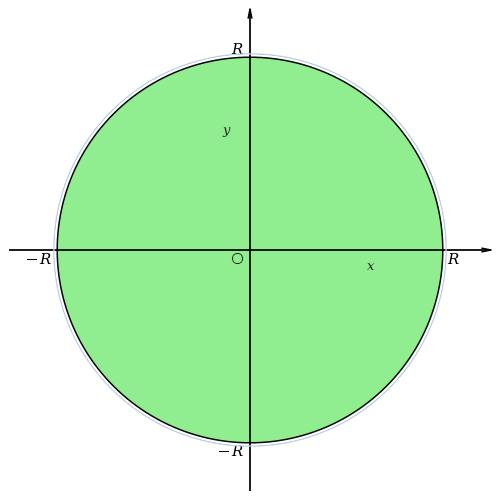
\includegraphics[width=0.2\paperwidth]{change_in_variables_polar_original_circle}
   \]
   &
   \[
   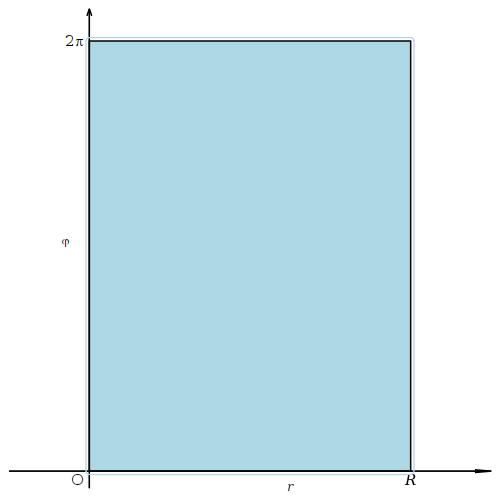
\includegraphics[width=0.2\paperwidth]{change_in_variables_polar_new_circle}
   \]\\
 \hline
   \[
   \left\{
   \begin{array}{c}
   x^2+y^2\leq R,\\
   y\geq 0
   \end{array}
   \right.
   \]
   &
   \[
   \left\{
   \begin{array}{c}
   0\leq r \leq R, \\
   0 \leq \varphi \leq \pi
   \end{array}
   \right.
   \]
   \\*
   \[
   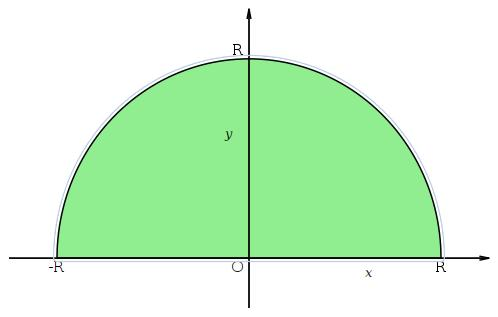
\includegraphics[width=0.2\paperwidth]{change_in_variables_polar_original_upper_semicircle}
   \]
   &
   \[
   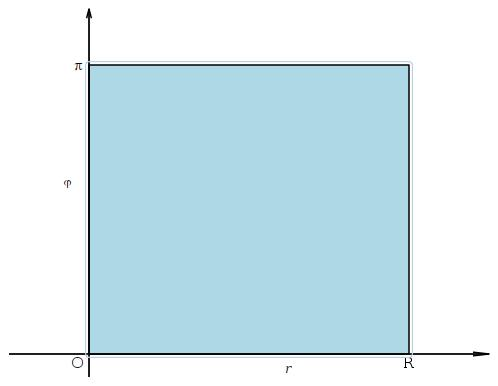
\includegraphics[width=0.2\paperwidth]{change_in_variables_polar_new_upper_semicircle}
   \]
   \\
 \hline
   \[
   \left\{
   \begin{array}{c}
   x^2+y^2\leq R,\\
   y\leq 0
   \end{array}
   \right.
   \]
   &
   \[
   \left\{
   \begin{array}{c}
   0\leq r \leq R, \\
   -\pi \leq \varphi \leq 0
   \end{array}
   \right.
   \]
   \\*
   \[
   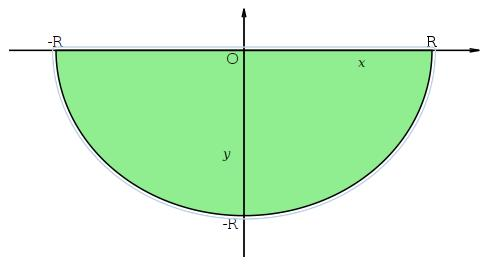
\includegraphics[width=0.2\paperwidth]{change_in_variables_polar_original_lower_semicircle}
   \]
   &
   \[
   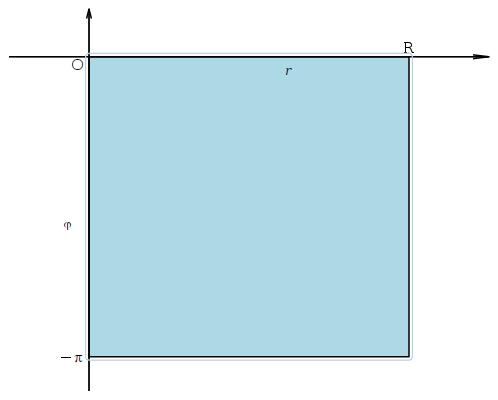
\includegraphics[width=0.2\paperwidth]{change_in_variables_polar_new_lower_semicircle}
   \]
   \\
 \hline
   \[
   \left\{
   \begin{array}{c}
   x^2+y^2\leq R,\\
   x\geq 0
   \end{array}
   \right.
   \]
   &
   \[
   \left\{
   \begin{array}{c}
   0\leq r \leq R, \\
   -\frac{\pi}{2} \leq \varphi \leq \frac{\pi}{2}
   \end{array}
   \right.
   \]
   \\*
   \[
   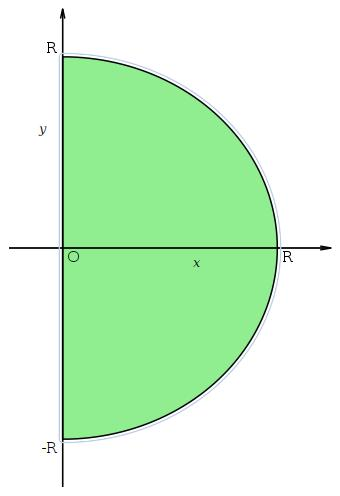
\includegraphics[width=0.2\paperwidth]{change_in_variables_polar_original_right_semicircle}
   \]
  &
   \[
   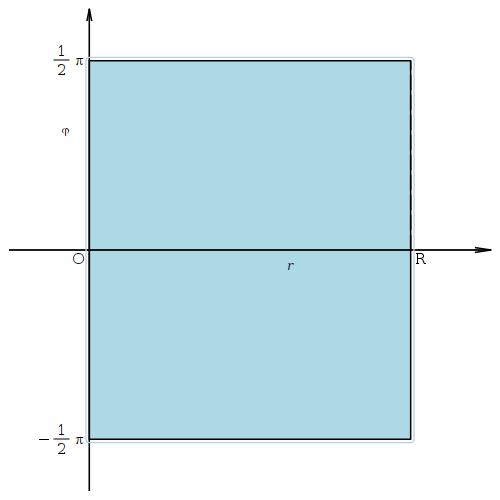
\includegraphics[width=0.2\paperwidth]{change_in_variables_polar_new_right_semicircle}
   \]
   \\
 \hline
 \[
   \left\{
   \begin{array}{c}
   x^2+y^2\leq R,\\
   x\leq 0
   \end{array}
   \right.
   \]
 &
 \[
   \left\{
   \begin{array}{c}
   0\leq r \leq R, \\
   \frac{\pi}{2}\leq \varphi \leq \frac{3\pi}{2}
   \end{array}
   \right.
   \]\\*
   \[
   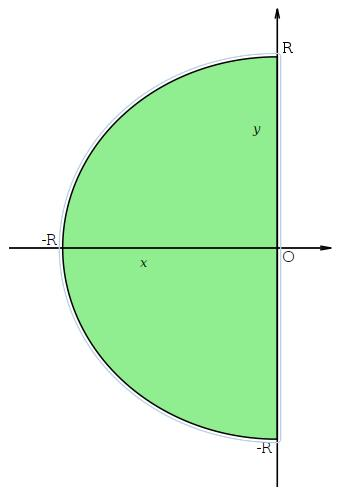
\includegraphics[width=0.2\paperwidth]{change_in_variables_polar_original_left_semicircle}
   \]
   &
   \[
   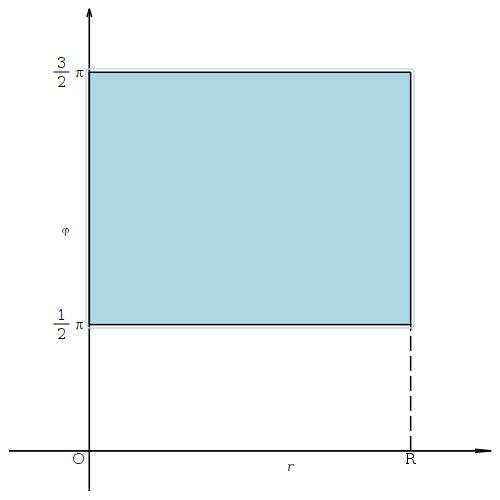
\includegraphics[width=0.2\paperwidth]{change_in_variables_polar_new_left_semicircle}
   \]
   \\
   \hline
   \[
   \left\{
   \begin{array}{c}
   x^2+y^2\leq R,\\
   x\geq 0,\\
   y\geq 0
   \end{array}
   \right.
   \]
   &
   \[
   \left\{
   \begin{array}{c}
   0\leq r \leq R, \\
   0 \leq \varphi \leq \frac{\pi}{2}
   \end{array}
   \right.
   \]
   \\*
   \[
   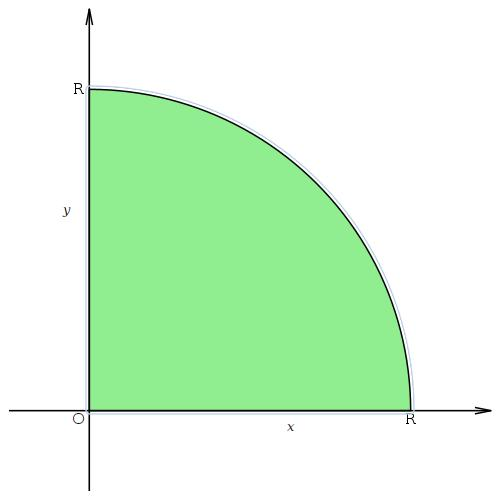
\includegraphics[width=0.2\paperwidth]{change_in_variables_polar_original_1st_quadrant}
   \]
   &
   \[
   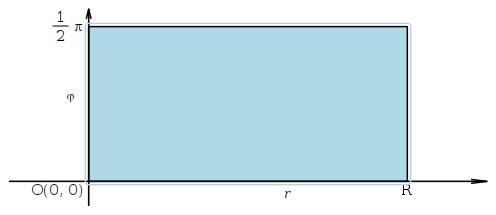
\includegraphics[width=0.2\paperwidth]{change_in_variables_polar_new_1st_quadrant}
   \]
   \\
   \hline
   \[
   \left\{
   \begin{array}{c}
   x^2+y^2\leq R,\\
   x\leq 0,\\
   y\geq 0
   \end{array}
   \right.
   \]
   &
   \[
   \left\{
   \begin{array}{c}
   0\leq r \leq R, \\
   \frac{\pi}{2} \leq \varphi \leq \pi
   \end{array}
   \right.
   \]
   \\*
   \[
   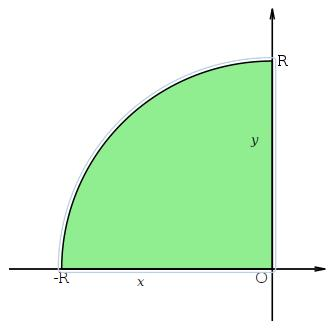
\includegraphics[width=0.2\paperwidth]{change_in_variables_polar_original_2nd_quadrant}
   \]
   &
   \[
   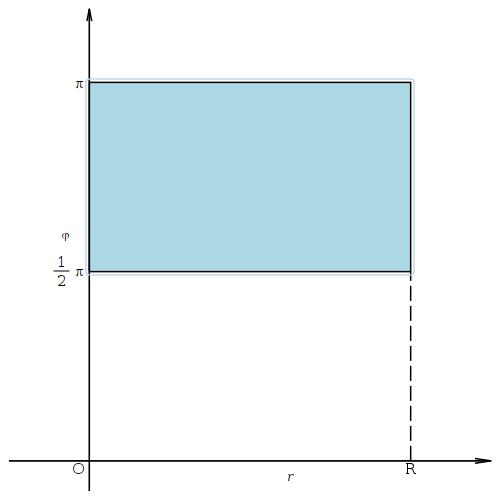
\includegraphics[width=0.2\paperwidth]{change_in_variables_polar_new_2nd_quadrant}
   \]
   \\
   \hline
   \[
   \left\{
   \begin{array}{c}
   x^2+y^2\leq R,\\
   x\leq 0,\\
   y\leq 0
   \end{array}
   \right.
   \]
   &
   \[
   \left\{
   \begin{array}{c}
   0\leq r \leq R, \\
   -\pi \leq \varphi \leq -\frac{\pi}{2}
   \end{array}
   \right.
   \]
   \\*
   \[
   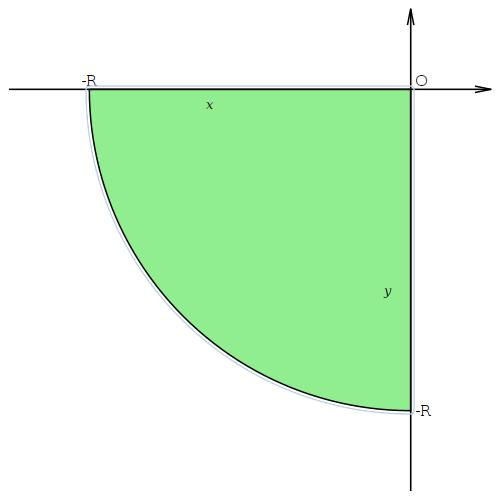
\includegraphics[width=0.2\paperwidth]{change_in_variables_polar_original_3rd_quadrant}
   \]
   &
   \[
   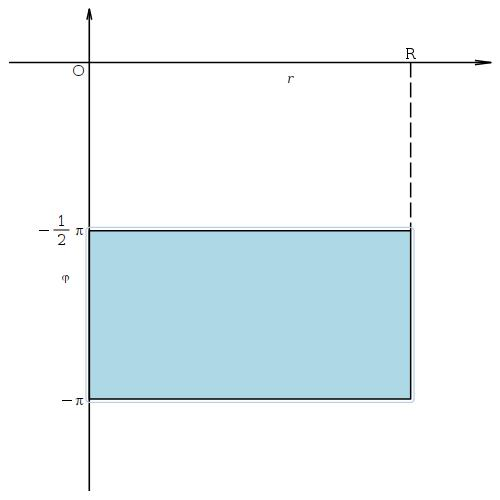
\includegraphics[width=0.2\paperwidth]{change_in_variables_polar_new_3rd_quadrant}
   \]
   \\
   \hline
   \[
   \left\{
   \begin{array}{c}
   x^2+y^2\leq R,\\
   x\geq 0,\\
   y\leq 0
   \end{array}
   \right.
   \]
   &
   \[
   \left\{
   \begin{array}{c}
   0\leq r \leq R, \\
   -\frac{\pi}{2} \leq \varphi \leq 0
   \end{array}
   \right.
   \]
   \\*
   \[
   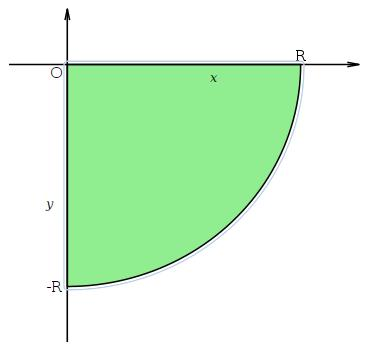
\includegraphics[width=0.2\paperwidth]{change_in_variables_polar_original_4th_quadrant}
   \]
   &
   \[
   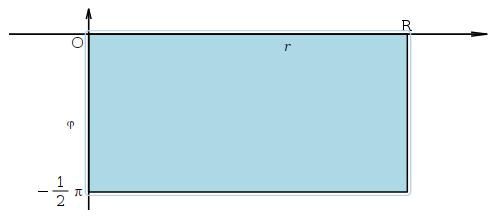
\includegraphics[width=0.2\paperwidth]{change_in_variables_polar_new_4th_quadrant}
   \]
   \\
   \hline
   \[
   \left\{
   \begin{array}{c}
   x^2+y^2\leq R_2,\\
   x^2+y^2\geq R_1,\\
   y\geq x\tg \alpha,\\
   y\geq x\tg \beta
   \end{array}
   \right.
   \]
   &
   \[
   \left\{
   \begin{array}{c}
   R_1\leq r \leq R_2, \\
   \alpha \leq \varphi \leq \beta
   \end{array}
   \right.
   \]
   \\*
   \[
   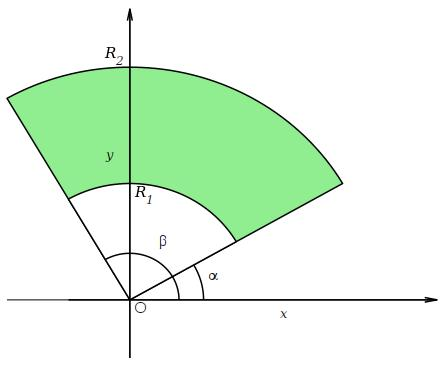
\includegraphics[width=0.2\paperwidth]{change_in_variables_polar_original_ring_sector}
   \]
   &
   \[
   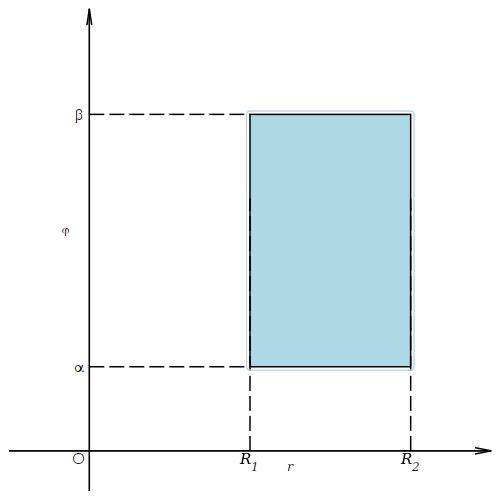
\includegraphics[width=0.2\paperwidth]{change_in_variables_polar_new_ring_sector}
   \]
   \\
   \hline
   \[
   \left\{
   \begin{array}{c}
   x^2+y^2\leq R,\\
   y\geq x\tg \alpha,\\
   y\geq x\tg \beta
   \end{array}
   \right.
   \]
   &
   \[
   \left\{
   \begin{array}{c}
   0\leq r \leq R, \\
   \alpha \leq \varphi \leq \beta
   \end{array}
   \right.
   \]
   \\*
   \[
   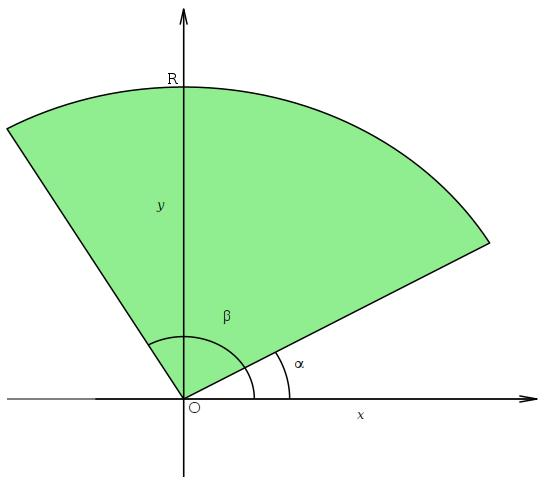
\includegraphics[width=0.2\paperwidth]{change_in_variables_polar_original_sector}
   \]
   &
   \[
   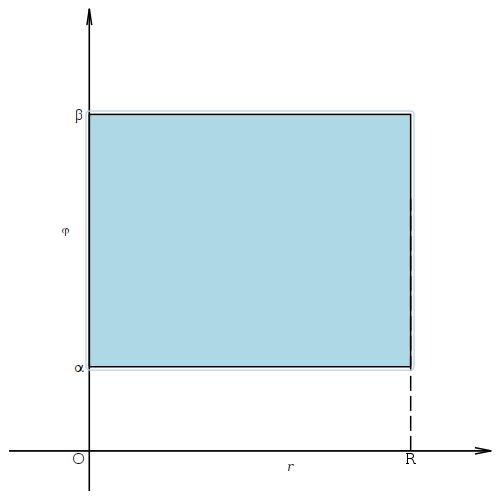
\includegraphics[width=0.2\paperwidth]{change_in_variables_polar_new_sector}
   \]
   \\
   \hline
 \end{longtable}

\subsection{Перехід до сферичних координат}
Перехід до сферичних координат може бути корисним у випадках, коли область інтегрування є тривимірною кулею, або її частиною --- кільцем, сектором, кільцевим сектором. Декартові початкові координати ${\left(x, y, z\right)}$ виражаються через нові сферичні координати ${\left(r, \varphi, \theta\right)}$ за допомогою перетворення $g$, що задається формулами
\[
\left(\begin{array}{c}x\\y\\z\end{array}\right) = g\left(r, \varphi, \theta\right) =
\left(
\begin{array}{c}
g_1\left(r,\varphi. \theta\right)\\
g_2\left(r,\varphi. \theta\right)\\
g_3\left(r,\varphi. \theta\right)\\
\end{array}
\right)=
\left(
\begin{array}{c}
r\cos\theta\cos\varphi\\
r\cos\theta\sin\varphi\\
r\sin\theta
\end{array}
\right),
\]
тобто
\begin{align*}
x = g_1\left(r, \varphi, \theta\right)= r \cos\theta \cos\varphi,\\
y = g_2\left(r, \varphi, \theta\right)= r \cos\theta \sin\varphi,\\
z = g_2\left(r, \varphi, \theta\right)= r \sin\theta.
\end{align*}
Якобіан при цьому дорівнює
\begin{align*}
&J(r, \varphi, \theta) = \dfrac{\partial\left(g_1,g_2,g_3\right)}{\partial\left(r,\varphi,\theta\right)} =
\begin{vmatrix}
\frac{\partial g_1}{\partial r} & \frac{\partial g_1}{\partial \varphi} & \frac{\partial g_1}{\partial \theta}\\[6pt]\frac{\partial g_2}{\partial r} & \frac{\partial g_2}{\partial \varphi} & \frac{\partial g_2}{\partial \theta}\\[6pt]\frac{\partial g_3}{\partial r} & \frac{\partial g_3}{\partial \varphi} & \frac{\partial g_3}{\partial \theta}
\end{vmatrix}
=
\begin{vmatrix}
\left(r \cos\theta \cos \varphi\right)'_{r} & \left(r \cos\theta \cos \varphi\right)'_{\varphi} & \left(r \cos\theta \cos \varphi\right)'_{\theta}\\[6pt]
\left(r \cos \theta \sin \varphi\right)'_{r} & \left(r \cos \theta \sin \varphi\right)'_{\varphi} & \left(r \cos\theta \sin \varphi\right)'_{\theta}\\[6pt]
\left(r \sin \theta\right)'_{r} & \left(r \sin \theta\right)'_{\varphi} & \left(r \sin\theta\right)'_{\theta}\end{vmatrix} = & \\[6pt]
&=
\begin{vmatrix}
\cos\theta \cos \varphi & - r \cos\theta \sin \varphi & - r \sin\theta \cos \varphi\\[6pt]
\cos \theta \sin \varphi & r \cos \theta \cos \varphi & - r \sin\theta \sin \varphi\\[6pt]
\sin \theta & 0 & r \cos\theta
\end{vmatrix}
= \underline{r^2 \cos^2 \varphi \cos^3 \theta} + \underline{\underline{r^2 \sin^2 \varphi \cos \theta \sin^2 \theta}} + & \\[6pt]
& + \underline{r^2 \cos^2 \varphi \sin^2\theta \cos \theta} + \underline{\underline{r^2 \cos^3 \theta \sin^2 \varphi}} = r^2 \cos^2 \varphi \cos \theta \left(\cos^2 \theta + \sin^2 \theta\right) +&\\[6pt]
&+r^2 \sin^2 \varphi \cos \theta \left(\sin^2 \theta +\cos^2 \theta\right) = r^2 \cos^2 \varphi \cos \theta + r^2 \sin^2 \varphi \cos \theta = r^2 \cos \theta \left(\cos^2 \varphi + \sin^2 \varphi \right) = &\\[6pt] & = r^2 \cos \theta.
\end{align*}

Формула заміни змінних в цьому випадку має наступний вигляд:
\begin{align*}
\boxed{\int\limits_{g\left(B\right)} f(x, y, z) dx dy dz = \int\limits_{B} f\left(r \cos\theta \cos\varphi, r \cos\theta \sin\varphi, r \sin\theta \right) r^2 \cos \theta dr d\varphi d\theta.}
\end{align*}
\subsection{Перехід до циліндричних координат}
Перехід до циліндричних координат може бути корисним у випадках, коли область інтегрування є тривимірною циліндричною областю з колом, або його частиною --- кільцем, сектором, кільцевим сектором --- в основі. Декартові початкові координати ${\left(x, y, z\right)}$ виражаються через нові циліндричні координати ${\left(r, \varphi, z\right)}$ за допомогою перетворення $g$, що задається формулами
\[
\left(\begin{array}{c}x\\y\\z\end{array}\right) = g\left(r, \varphi, \theta\right) =
\left(
\begin{array}{c}
g_1\left(r,\varphi. z\right)\\
g_2\left(r,\varphi. z\right)\\
g_3\left(r,\varphi. z\right)\\
\end{array}
\right)=
\left(
\begin{array}{c}
r \cos\varphi\\
r \sin\varphi\\
z
\end{array}
\right),
\]
тобто
\begin{align*}
x = g_1\left(r, \varphi, z\right)= r \cos\varphi,\\
y = g_2\left(r, \varphi, z\right)= r \sin\varphi,\\
z = g_2\left(r, \varphi, z\right)= z.
\end{align*}
Якобіан при цьому дорівнює
\begin{align*}
&J(r, \varphi, z) = \dfrac{\partial\left(g_1,g_2,g_3\right)}{\partial\left(r,\varphi,z\right)} =
\begin{vmatrix}
\frac{\partial g_1}{\partial r} & \frac{\partial g_1}{\partial \varphi} & \frac{\partial g_1}{\partial z}\\[6pt]\frac{\partial g_2}{\partial r} & \frac{\partial g_2}{\partial \varphi} & \frac{\partial g_2}{\partial z}\\[6pt]\frac{\partial g_3}{\partial r} & \frac{\partial g_3}{\partial \varphi} & \frac{\partial g_3}{\partial z}
\end{vmatrix}
=
\begin{vmatrix}
\left(r \cos \varphi\right)'_{r} & \left(r \cos \varphi\right)'_{\varphi} & \left(r \cos \varphi\right)'_{z}\\[6pt]
\left(r \sin \varphi\right)'_{r} & \left(r \sin \varphi\right)'_{\varphi} & \left(r \sin \varphi\right)'_{z}\\[6pt]
\left(z \right)'_{r} & \left(z \right)'_{\varphi} & \left(z\right)'_{z}\end{vmatrix} = & \\[6pt]
&=
\begin{vmatrix}
 \cos \varphi & - r \sin \varphi & 0\\[6pt]
 \sin \varphi & r \cos \varphi & 0\\[6pt]
0 & 0 & 1
\end{vmatrix}
= r \cos^2 \varphi + r \sin^2 \varphi = r.
\end{align*}

Формула заміни змінних в цьому випадку має наступний вигляд:
\begin{align*}
\boxed{\int\limits_{g\left(B\right)} f(x, y, z) dx dy dz = \int\limits_{B} f\left(r \cos\varphi, r \sin\varphi, z \right) r dr d\varphi dz.}
\end{align*}
\section{Приклади обчислень}
\begin{example}[перехід до полярних координат]
Знайти ${\iint\limits_D x y d x d y}$, де через $D$ позначена область в першому квадранті ${x\geq0}$, ${y\geq0}$, що обмежена лініями ${x^2 +y^2 = R^2}$, ${y= 0}$, ${y = x\sqrt{3}}$.
\end{example}
Зробимо рисунок почактової області $D$ (нагадаємо, що ${\sqrt{3} = \tg \frac{\pi}{3}}$):
\[
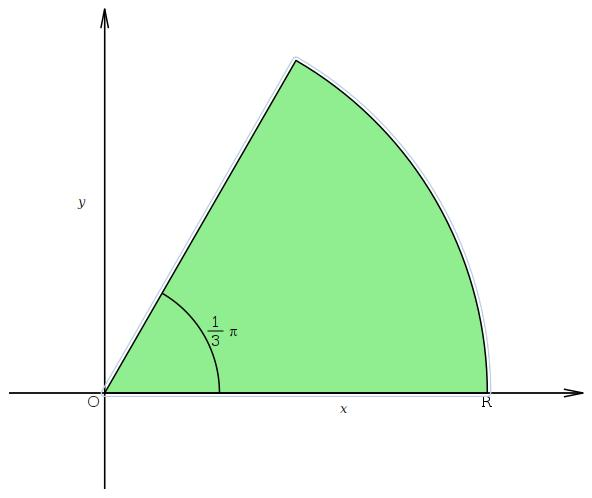
\includegraphics[width=0.3\paperwidth]{change_in_variables_example_polar_original}
\]
Після переходу до полярних координат нова область $D'$ виглядає наступним чином:
\[
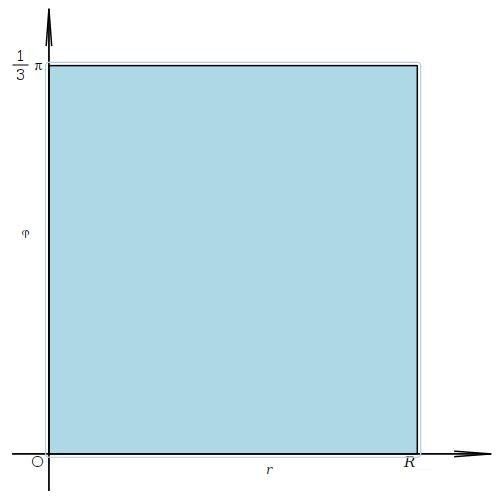
\includegraphics[width=0.3\paperwidth]{change_in_variables_example_polar_new}
\]

\begin{align*}
&\iint\limits_D x y d x d y = \iint\limits_{D'} r \cos \varphi r \cdot \sin \varphi \cdot r d r d \varphi = \int\limits_{0}^{R}\left(\int\limits_{0}^{\frac{\pi}{3}}r^3 \cos \varphi \sin \varphi d \varphi\right) d r =&\\
&= \int\limits_{0}^{R}\left(\frac{1}{2}\int\limits_{0}^{\frac{\pi}{3}}r^3 \sin 2 \varphi d \varphi\right) d r = \int\limits_{0}^{R}\frac{1}{2}\left(-\frac{1}{2}r^3 \cos 2 \varphi \biggr|_{\varphi = 0}^{\frac{\pi}{3}} \right) d r = &\\
&= \int\limits_{0}^{R}\left(-\frac{1}{4}r^3 \cos 2 \frac{\pi}{3} - \left(-\frac{1}{4}r^3 \cos 0\right) \right) d r = \int\limits_{0}^{R}\left(\frac{1}{8}r^3 - \left(-\frac{1}{4}r^3 \right) \right) d r = &\\
& = \int\limits_{0}^{R}\frac{3}{8}r^3 d r = \frac{3}{8}\cdot\frac{r^4}{4}\biggr|_{0}^{R} = \frac{3 R^4}{32} - 0 = \frac{3 R^4}{32}.&
\end{align*}
\begin{example}[Загальна формула]
Знайти ${\iint\limits_D \ln\left(x + y\right) d x d y}$, де через $D$ позначений паралелограм, що обмежений прямими ${x - 3y + 7 = 0}$, ${x - 3y + 2 = 0}$, ${2x - y - 1 = 0}$, ${2x - y - 6 = 0}$.

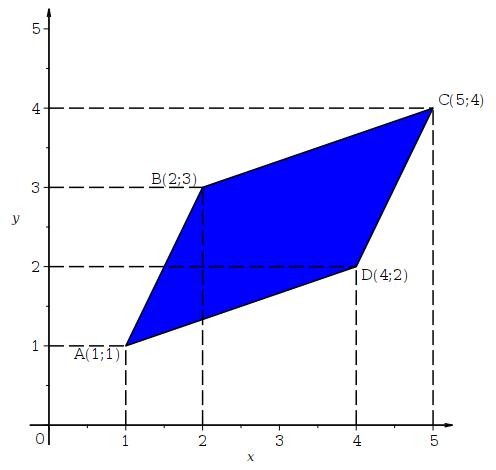
\includegraphics[width=0.5\paperwidth]{example.2.6}

Як і в попередніх прикладах, область $D$ є множиною на площині циліндричною в напрямку осі ${Oy}$. Однак тепер, якщо безпосередньо зводити подвійний інтеграл до повторного, то ми отримаємо суму не двох, а трьох повторних інтегралів:
\[
\begin{array}{l}
\iint\limits_D \ln\left(x + y\right) d x d y =\\= \int\limits_1^2 d x \int\limits_{\frac{x+2}{3}}^{2 x - 1}\ln\left(x + y\right) d y + \int\limits_2^4 d x\int\limits_{\frac{x+2}{3}}^{\frac{x + 7}{3}}\ln\left(x + y\right) d y + \int\limits_4^5 d x\int\limits_{2 x - 6}^{\frac{x + 7}{3}}\ln\left(x + y\right) d y.
\end{array}
\]
\begin{exercise}
Підрахуйте ці повторні інтеграли і переконайтесь, що в сумі ви отримали таку саму відповідь, яку ми отримаємо нижче за допомогою заміни змінних.
\end{exercise}
\begin{exercise}
Зведіть даний в умові подвійний інтеграл до суми трьох повторних на підставі того, що $D$ є множиною циліндричною в напрямку також осі ${Ox}$.
\end{exercise}
Розглянемо нові змінні
\[
\begin{array}{c}
s = 3 y - x,\\
t = 2 x - y.
\end{array}
\]
Фактично ми задали перетворення ${h\colon \eucl{2}\to\eucl{2}}$, яке точку ${\left(x, y\right)\in\eucl{2}}$
 переводить в точку ${\left(s,t\right) = h\left(x,y\right)\in\eucl{2}}$ за наведеними вище формулами. В геометрії такі пертворення називаються афінними. Відомо, що афінні перетворення зберігають паралельність прямих, а тому переводять паралелограми в паралелограми. В нашому випадку область $D$ є паралелограмом з вершинами ${\left(1,1\right)}$, ${\left(2,3\right)}$, ${\left(5,4\right)}$ і ${\left(4,2\right)}$. Знайдемо тепер, в які точки переводить перетворення $h$ вершини нашого паралелограма:
 \[
 \begin{array}{c}
 h\left(1,1\right) = \left(\begin{array}{c}3\cdot1 - 1\\2\cdot 1 - 1\end{array}\right) = \left(\begin{array}{c}2\\1\end{array}\right),\\
 h\left(2,3\right) = \left(\begin{array}{c}3\cdot3 - 2\\2\cdot 2 - 3\end{array}\right) = \left(\begin{array}{c}7\\1\end{array}\right),\\
 h\left(5,4\right) = \left(\begin{array}{c}3\cdot4 - 5\\2\cdot 5 - 4\end{array}\right) = \left(\begin{array}{c}7\\6\end{array}\right),\\
 h\left(4,2\right) = \left(\begin{array}{c}3\cdot2 - 4\\2\cdot 4 - 2\end{array}\right) = \left(\begin{array}{c}2\\6\end{array}\right),\\
 \end{array}
 \]

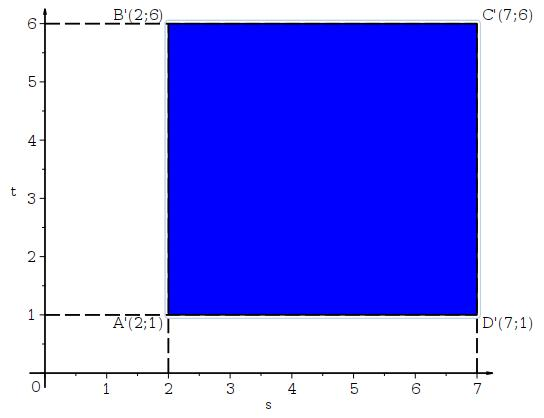
\includegraphics[width=0.3\paperwidth]{example.2.6_1}

Таким чином, область ${D' = h\left(D\right)}$, що є образом області $D$ під дією перетворення $g$, є паралелограм, а фактично --- прямокутник, з вершинами $\left(2,1\right)$, $\left(7,1\right)$, $\left(7,6\right)$ і $\left(2,6\right)$

Для того, щоб застосувати формулу заміни змінних, нам потрібне обернене перетворення $g$. Для того, щоб його отримати, потрібно змінні $x$ і $y$ виразити через змінні $s$ і $t$:

\[
\begin{array}c
\left\{
\begin{array}{l}
s = 3 y - x,\\
t = 2 x - y
\end{array}
\right.
\Leftrightarrow
\left\{
\begin{array}{l}
x = 3 y - s,\\
t = 2 x - y
\end{array}
\right.
\Leftrightarrow
\left\{
\begin{array}{l}
x = 3 y - s,\\
t = 2 \cdot (3 y - s) - y
\end{array}
\right.
\Leftrightarrow
\\[20pt]
\Leftrightarrow
\left\{
\begin{array}{l}
x = 3 y - s,\\
t = 6 y - 2 s - y
\end{array}
\right.
\Leftrightarrow
\left\{
\begin{array}{l}
x = 3 y - s,\\
t = 5 y - 2 s
\end{array}
\right.
\Leftrightarrow
\left\{
\begin{array}{l}
x = 3 y - s,\\
5 y = t + 2 s
\end{array}
\right.
\Leftrightarrow
\\[20pt]
\Leftrightarrow
\left\{
\begin{array}{l}
x = 3 y - s,\\[6pt]
y = \frac{t + 2 s}{5}
\end{array}
\right.
\Leftrightarrow
\left\{
\begin{array}{l}
x = 3 \cdot \frac{t + 2 s}{5} - s,\\[6pt]
y = \frac{t + 2 s}{5}
\end{array}
\right.
\Leftrightarrow
\left\{
\begin{array}{l}
x = \frac{s + 3 t}{5},\\[6pt]
y = \frac{t + 2 s}{5}
\end{array}
\right.
\end{array}
\]
Таким чином, перетворення $g$, обернене до пертворення $h$, задається формулами
\[
\begin{array}{l}
x = \frac{s + 3 t}{5},\\
y = \frac{t + 2 s}{5}.
\end{array}
\]
Знайдемо тепер якобіан:
\[
\begin{array}{c}
J(s, t) = g'(s, t) = \frac{\partial\left(g_1, g_2\right)}{\partial\left(s, t\right)} =
\left|
\begin{array}{cc}
\frac{\partial g_1}{\partial s} & \frac{\partial g_1}{\partial t}\\[6pt]
\frac{\partial g_2}{\partial s} & \frac{\partial g_2}{\partial t}
\end{array}
\right|
=
\begin{vmatrix}
\frac{\partial}{\partial s}\left(\frac{s + 3 t}{5}\right) & \frac{\partial }{\partial t}\left(\frac{s + 3 t}{5}\right)\\[6pt]
\frac{\partial }{\partial s}\left(\frac{t + 2 s}{5}\right) & \frac{\partial }{\partial t}\left(\frac{t + 2 s}{5}\right)
\end{vmatrix}
=\\
=
\left|
\begin{array}{cc}
\frac{1}{5} & \frac{3}{5}\\[6pt]
\frac{2}{5} & \frac{1}{5}
\end{array}
\right|
= \frac{1}{5} \cdot \frac{1}{5} - \frac{3}{5}\cdot \frac{2}{5} = \frac{1}{25} - \frac{6}{25} = -\frac{5}{25} = -\frac{1}{5}.
\end{array}
\]
Згідно з формулою заміни змінних маємо
\[
\begin{array}{c}
\iint\limits_D \ln\left(x + y\right) d x d y = \iint\limits_{D'} \ln\left(\frac{s + 3 t}{5} + \frac{t + 2 s}{5}\right) \cdot\left| -\frac{1}{5} \right| d s d t = \frac{1}{5} \iint\limits_{D'} \ln\frac{3 s + 4 t}{5} d s d t.
\end{array}
\]
Тепер підрахуємо подвійний інтеграл
\[
\iint\limits_{D'} \ln\frac{3 s + 4 t}{5} d s d t.
\]
Оскільки логарифм частки є різницею логарифмів, маємо
\[
\ln\frac{3 s + 4 t}{5} = \ln\left(3 s + 4 t\right) - \ln 5,
\]
і, на підставі лінійності кратних інтегралів,
\[
\iint\limits_{D'} \ln\frac{3 s + 4 t}{5} d s d t = \iint\limits_{D'} \ln\left(3 s + 4 t\right) d s d t - \iint\limits_{D'} \ln 5 d s d t
\]

Інтеграл від константи дорівнює константі, помноженій на міру області інтегрування. В нашому випадку $D'$ є прямокутником, його міра є його площею:
\[
m\left(D'\right) = 5\cdot 5 = 25,
\]
і
\[
\iint\limits_{D'} \ln 5 d s d t = 25\ln 5.
\]
Тепер ми маємо підрахувати подвійний інтеграл
\[
\iint\limits_{D'} \ln\left(3 s + 4 t\right) d s d t.
\]
Останній подвійний інтеграл береться вздовж нової обдасті $D'$, яка є прямокутником, а тому він зводиться до простого повторного інтегралу:
\[
\iint\limits_{D'}\ln\left(3 s + 4 t\right) d s d t = \int\limits_2^7 d s \int\limits_1^6\ln\left(3 s + 4 t\right) d t.
\]
Підрахуємо спочатку
\[
\int\limits_1^6\ln\left(3 s + 4 t\right) d t.
\]
Інтеграл від логарифма рахується за допомогою інтегрування частинами
\[
\int\limits_a^b u dv = u v \biggr|_a^b - \int\limits_a^b v du,
\]
але для спрощення подальших обчислень варто спочатку зробити заміну змінної:
\begin{align*}
&\int\limits_1^6\ln\left(3 s + 4 t\right) d t = &\\[6pt]
&\left(\begin{array}{c}\mbox{ заміна }\\ \mbox{ змінної }\end{array}\right)\left[\begin{array}{c}z = 3 s + 4 t \Leftrightarrow t = \frac{z - 3 s}{4} \\[6pt] dt = \left(\frac{z - 3 s}{4}\right)'_zdz = \frac{dz}{4} \end{array}\ \begin{array}{|c|c|}\hline t&z\\\hline 6&3 s + 24\\\hline 1&3 s + 4\\\hline \end{array}\ \right] = \frac{1}{4}\int\limits_{3 s + 4}^{3 s + 24} \ln z d z = &\\[6pt]
&\left(\begin{array}{c}\mbox{ інтегрівання }\\ \mbox{ частинами }\end{array}\right)\left[\begin{array}{ll}u = \ln z & \ \ \ d v = d z\\ d u = \left(\ln z\right)'d z = \frac{dz }{z} & \ \ \ v = \int dz = z\end{array}\right] = &\\[6pt]
&=\frac{1}{4}\left( z\ln z \biggr|_{3 s + 4}^{3 s + 24} - \int\limits_{3 s + 4}^{3 s + 24}z\cdot\frac{d z}{z}\right) = & \\[6pt]
&\mbox{(підстановка)} &\\[6pt]
&=\frac{1}{4}\left(\left(3 s + 24\right)\ln\left(3 s + 24\right) - \left(3 s + 4\right)\ln\left(3 s + 4\right) - \int\limits_{3 s + 4}^{3 s + 24} d z\right) = & \\[6pt]
&\mbox{(інтеграл від константи)} &\\[6pt]
&=\frac{1}{4}\left(\left(3 s + 24\right)\ln\left(3 s + 24\right) - \left(3 s + 4\right)\ln\left(3 s + 4\right) - \left(3 s + 24 - \left(3 s + 4\right)\right)\right) = & \\[6pt]
&=\frac{1}{4}\left(\left(3 s + 24\right)\ln\left(3 s + 24\right) - \left(3 s + 4\right)\ln\left(3 s + 4\right) - 20\right) &
\end{align*}

Тобто,
\[
\begin{array}{c}
\int\limits_1^6\ln\left(3 s + 4 t\right) d t = \frac{1}{4}\left(\left(3 s + 24\right)\ln\left(3 s + 24\right) - \left(3 s + 4\right)\ln\left(3 s + 4\right) - 20\right).
\end{array}
\]
Таким чином,
\begin{align*}
&\iint\limits_{D'}\ln\left(3 s + 4 t\right) d s d t =&\\
&= \int\limits_2^7 \frac{1}{4}\left(\left(3 s + 24\right)\ln\left(3 s + 24\right) - \left(3 s + 4\right)\ln\left(3 s + 4\right) - 20\right) d s =& \\[6pt]
&\mbox{(лінійність)} &\\[6pt]
&=\frac{1}{4}\int\limits_2^7 \left(\left(3 s + 24\right)\right)\ln\left(3 s + 24\right) d s - \frac{1}{4}\int\limits_2^7 \left(\left(3 s + 4\right)\right) \ln\left(3 s + 4\right) d s - 5 \int\limits_{2}^{7}d s &
\end{align*}
Останній інтеграл від константи, в данному випадку одиниці, дорівнює константі, домноженій на міру множини, тобто, в данному випадку, на довжину проміжка:
\[
 \int\limits_{2}^{7}d s = 1 \cdot \left(7 - 2\right) = 5.
\]
Перші два інтеграли рахуються за допомогою інтегрування частинами. В кожному з них для спрощення обчислень варто спочатку зробити заміну змінної.
\begin{align*}
&\int\limits_2^7 \left(3 s + 24\right)\ln\left(3 s + 24\right) d s = &\\[6pt]
&\left(\begin{array}{c}\mbox{ заміна }\\ \mbox{ змінної }\end{array}\right)\left[\begin{array}{c}z = 3 s + 24 \Leftrightarrow s = \frac{z - 24}{3} \\[6pt] ds = \left(\frac{z - 24}{3}\right)'dz = \frac{dz}{3} \end{array}\ \begin{array}{|c|c|}\hline s&z\\\hline 7 & 45\\\hline 2&30\\\hline \end{array}\ \right] = \frac{1}{3}\int\limits_{30}^{45}z \ln z d z = &\\[6pt]&\left(\begin{array}{c}\mbox{ інтегрівання }\\ \mbox{ частинами }\end{array}\right)\left[\begin{array}{ll}u = \ln z & \ \ \ dv = z d z\\ du = \left(\ln z\right)'dz = \frac{dz}{z} & \ \ \ v = \int z d z = \frac{z^2}{2}\end{array}\right] = &\\[6pt]
&= \frac{1}{3}\left(\frac{z^2}{2}\ln z \biggr|_{30}^{45} - \int\limits_{30}^{45}\frac{z^2}{2}\frac{d z}{z}\right) = & \\[6pt]
&\mbox{(підстановка)} &\\[6pt]
&=\frac{1}{3}\left(\ln 45\cdot \frac{45^2}{2} - \ln 30\cdot \frac{30^2}{2} - \int\limits_{30}^{45}\frac{z}{2} d z =\right)&\\[6pt]
&=\frac{1}{3}\left( \frac{2025}{2}\ln \left(5\cdot 3^2\right) - 450\ln \left(2 \cdot 3 \cdot 5\right) - \int\limits_{30}^{45}\frac{z}{2}d z\right) =&\\[6pt]
&=\frac{1}{3}\left(\frac{2025}{2}\ln 5 + 2025\ln 3 - 450\ln 2 - 450\ln 3 -450 \ln 5 - \frac{z^2}{4}\biggr|_{30}^{45}\right) = &\\[6pt]
&= \frac{1}{3}\left(\frac{1125}{2}\ln 5 + 1575\ln 3 - 450\ln 2 - \left(\frac{45^2}{4} - \frac{30^2}{4} \right)\right) = & \\[6pt]
&=\frac{1}{3}\left( \frac{1125}{2}\ln 5 + 1575\ln 3 - 450\ln 2 - \frac{1125}{4}\right) = & \\[6pt]
&= \frac{375}{2}\ln 5 + 525\ln 3 - 150\ln 2 - \frac{375}{4}.&
\end{align*}
\begin{align*}
&\int\limits_2^7 \left(3 s + 4\right)\ln\left( s + 24\right) d s = &\\[6pt]
&\left(\begin{array}{c}\mbox{ заміна }\\ \mbox{ змінної }\end{array}\right)\left[\begin{array}{c}z = s + 24 \Leftrightarrow s = \frac{z - 4}{3} \\[6pt] ds = \left(\frac{z - 4}{3}\right)'dz = \frac{dz}{3} \end{array}\ \begin{array}{|c|c|}\hline s&z\\\hline 7 & 25\\\hline 2&10\\\hline \end{array}\ \right] = \frac{1}{3}\int\limits_{10}^{25}z \ln z d z = &\\[6pt]&\left(\begin{array}{c}\mbox{ інтегрівання }\\ \mbox{ частинами }\end{array}\right)\left[\begin{array}{ll}u = \ln z & \ \ \ dv = z d z\\ du = \left(\ln z\right)'dz = \frac{dz}{z} & \ \ \ v = \int z d z = \frac{z^2}{2}\end{array}\right] = &\\[6pt]
&= \frac{1}{3}\left(\frac{z^2}{2}\ln z \biggr|_{10}^{25} - \int\limits_{10}^{25}\frac{z^2}{2}\frac{d z}{z}\right) = & \\[6pt]
&\mbox{(підстановка)} &\\[6pt]
&=\frac{1}{3}\left(\ln 25\cdot \frac{25^2}{2} - \ln 10\cdot \frac{10^2}{2} - \int\limits_{10}^{25}\frac{z}{2} d z =\right)&\\[6pt]
&=\frac{1}{3}\left( \frac{625}{2}\ln \left(5^2\right) - 50\ln \left(2 \cdot 5\right) - \int\limits_{10}^{25}\frac{z}{2}d z\right) =&\\[6pt]
&=\frac{1}{3}\left(625\ln 5 - 50\ln 2 - 50 \ln 5 - \frac{z^2}{4}\biggr|_{10}^{25}\right) = &\\[6pt]
&= \frac{1}{3}\left(575\ln 5 - 50\ln 2 - \left(\frac{25^2}{4} - \frac{10^2}{4} \right)\right) = & \\[6pt]
&=\frac{1}{3}\left( 575\ln 5 - 50\ln 2 - \frac{525}{4}\right) = & \\[6pt]
&= \frac{575}{3}\ln 5 - \frac{50}{3}\ln 2 - \frac{175}{4}.&
\end{align*}

Тобто
\begin{align*}
&\int\limits_2^7 \left(3 s + 4\right)\ln\left( s + 24\right) d s = \frac{575}{3}\ln 5 - \frac{50}{3}\ln 2 - \frac{175}{4}.&
\end{align*}

Далі маємо
\begin{align*}
& \iint\limits_{D'}\ln\left(3 s + 4 t\right) d s d t = &\\[6pt]
&= \frac{1}{4}\left(\frac{375}{2}\ln 5 + 525\ln 3 - 150\ln 2 - \frac{375}{4}\right) - \frac{1}{4}\left(\frac{575}{3}\ln 5 - \frac{50}{3}\ln 2 - \frac{175}{4}\right) - 5 \cdot 5 = &\\[6pt]
&=-\frac{25}{24}\ln 5 + \frac{525}{4}\ln 3- \frac{100}{3}\ln 2 - \frac{75}{2},
\end{align*}
потім
\begin{align*}
& \iint\limits_{D'} \ln\frac{3 s + 4 t}{5} d s d t = &\\[6pt]
&=-\frac{25}{24}\ln 5 + \frac{525}{4}\ln 3- \frac{100}{3}\ln 2 - \frac{75}{2} - 25\ln 5 = &\\[6pt]
&=-\frac{625}{24}\ln 5 + \frac{525}{4}\ln 3- \frac{100}{3}\ln 2 - \frac{75}{2},
\end{align*}
і остаточно
\begin{align*}
& \iint\limits_D \ln\left(x + y\right) d x d y = &\\[6pt]
&=\frac{1}{5}\cdot\left(-\frac{625}{24}\ln 5 + \frac{525}{4}\ln 3- \frac{100}{3}\ln 2 - \frac{75}{2}\right) = -\frac{125}{24}\ln 5 + \frac{105}{4}\ln 3- \frac{20}{3}\ln 2 - \frac{15}{2}.
\end{align*}


\end{example}



















%
%
% \part{Part One}
%
% %----------------------------------------------------------------------------------------
% %	CHAPTER 1
% %----------------------------------------------------------------------------------------
%
% \chapterimage{chapter_head_2.pdf} % Chapter heading image
%
% \chapter{Text Chapter}
%
% \section{Paragraphs of Text}\index{Paragraphs of Text}
%
% \lipsum[1-7] % Dummy text
%
% %------------------------------------------------
%
% \section{Citation}\index{Citation}
%
% This statement requires citation \cite{article_key}; this one is more specific \cite[162]{book_key}.
%
% %------------------------------------------------
%
% \section{Lists}\index{Lists}
%
% Lists are useful to present information in a concise and/or ordered way\footnote{Footnote example...}.
%
% \subsection{Numbered List}\index{Lists!Numbered List}
%
% \begin{enumerate}
% \item The first item
% \item The second item
% \item The third item
% \end{enumerate}
%
% \subsection{Bullet Points}\index{Lists!Bullet Points}
%
% \begin{itemize}
% \item The first item
% \item The second item
% \item The third item
% \end{itemize}
%
% \subsection{Descriptions and Definitions}\index{Lists!Descriptions and Definitions}
%
% \begin{description}
% \item[Name] Description
% \item[Word] Definition
% \item[Comment] Elaboration
% \end{description}
%
% %----------------------------------------------------------------------------------------
% %	CHAPTER 2
% %----------------------------------------------------------------------------------------
%
% \chapter{In-text Elements}
%
% \section{Theorems}\index{Theorems}
%
% This is an example of theorems.
%
% \subsection{Several equations}\index{Theorems!Several Equations}
% This is a theorem consisting of several equations.
%
% \begin{theorem}[Name of the theorem]
% In $E=\mathbb{R}^n$ all norms are equivalent. It has the properties:
% \begin{align}
% & \big| ||\mathbf{x}|| - ||\mathbf{y}|| \big|\leq || \mathbf{x}- \mathbf{y}||\\
% &  ||\sum_{i=1}^n\mathbf{x}_i||\leq \sum_{i=1}^n||\mathbf{x}_i||\quad\text{where $n$ is a finite integer}
% \end{align}
% \end{theorem}
%
% \subsection{Single Line}\index{Theorems!Single Line}
% This is a theorem consisting of just one line.
%
% \begin{theorem}
% A set $\mathcal{D}(G)$ in dense in $L^2(G)$, $|\cdot|_0$.
% \end{theorem}
%
% %------------------------------------------------
%
% \section{Definitions}\index{Definitions}
%
% This is an example of a definition. A definition could be mathematical or it could define a concept.
%
% \begin{definition}[Definition name]
% Given a vector space $E$, a norm on $E$ is an application, denoted $||\cdot||$, $E$ in $\mathbb{R}^+=[0,+\infty[$ such that:
% \begin{align}
% & ||\mathbf{x}||=0\ \Rightarrow\ \mathbf{x}=\mathbf{0}\\
% & ||\lambda \mathbf{x}||=|\lambda|\cdot ||\mathbf{x}||\\
% & ||\mathbf{x}+\mathbf{y}||\leq ||\mathbf{x}||+||\mathbf{y}||
% \end{align}
% \end{definition}
%
% %------------------------------------------------
%
% \section{Notations}\index{Notations}
%
% \begin{notation}
% Given an open subset $G$ of $\mathbb{R}^n$, the set of functions $\varphi$ are:
% \begin{enumerate}
% \item Bounded support $G$;
% \item Infinitely differentiable;
% \end{enumerate}
% a vector space is denoted by $\mathcal{D}(G)$.
% \end{notation}
%
% %------------------------------------------------
%
% \section{Remarks}\index{Remarks}
%
% This is an example of a remark.
%
% \begin{remark}
% The concepts presented here are now in conventional employment in mathematics. Vector spaces are taken over the field $\mathbb{K}=\mathbb{R}$, however, established properties are easily extended to $\mathbb{K}=\mathbb{C}$.
% \end{remark}
%
% %------------------------------------------------
%
% \section{Corollaries}\index{Corollaries}
%
% This is an example of a corollary.
%
% \begin{corollary}[Corollary name]
% The concepts presented here are now in conventional employment in mathematics. Vector spaces are taken over the field $\mathbb{K}=\mathbb{R}$, however, established properties are easily extended to $\mathbb{K}=\mathbb{C}$.
% \end{corollary}
%
% %------------------------------------------------
%
% \section{Propositions}\index{Propositions}
%
% This is an example of propositions.
%
% \subsection{Several equations}\index{Propositions!Several Equations}
%
% \begin{proposition}[Proposition name]
% It has the properties:
% \begin{align}
% & \big| ||\mathbf{x}|| - ||\mathbf{y}|| \big|\leq || \mathbf{x}- \mathbf{y}||\\
% &  ||\sum_{i=1}^n\mathbf{x}_i||\leq \sum_{i=1}^n||\mathbf{x}_i||\quad\text{where $n$ is a finite integer}
% \end{align}
% \end{proposition}
%
% \subsection{Single Line}\index{Propositions!Single Line}
%
% \begin{proposition}
% Let $f,g\in L^2(G)$; if $\forall \varphi\in\mathcal{D}(G)$, $(f,\varphi)_0=(g,\varphi)_0$ then $f = g$.
% \end{proposition}
%
% %------------------------------------------------
%
% \section{Examples}\index{Examples}
%
% This is an example of examples.
%
% \subsection{Equation and Text}\index{Examples!Equation and Text}
%
% \begin{example}
% Let $G=\{x\in\mathbb{R}^2:|x|<3\}$ and denoted by: $x^0=(1,1)$; consider the function:
% \begin{equation}
% f(x)=\left\{\begin{aligned} & \mathrm{e}^{|x|} & & \text{si $|x-x^0|\leq 1/2$}\\
% & 0 & & \text{si $|x-x^0|> 1/2$}\end{aligned}\right.
% \end{equation}
% The function $f$ has bounded support, we can take $A=\{x\in\mathbb{R}^2:|x-x^0|\leq 1/2+\epsilon\}$ for all $\epsilon\in\intoo{0}{5/2-\sqrt{2}}$.
% \end{example}
%
% \subsection{Paragraph of Text}\index{Examples!Paragraph of Text}
%
% \begin{example}[Example name]
% \lipsum[2]
% \end{example}
%
% %------------------------------------------------
%
% \section{Exercises}\index{Exercises}
%
% This is an example of an exercise.
%
% \begin{exercise}
% This is a good place to ask a question to test learning progress or further cement ideas into students' minds.
% \end{exercise}
%
% %------------------------------------------------
%
% \section{Problems}\index{Problems}
%
% \begin{problem}
% What is the average airspeed velocity of an unladen swallow?
% \end{problem}
%
% %------------------------------------------------
%
% \section{Vocabulary}\index{Vocabulary}
%
% Define a word to improve a students' vocabulary.
%
% \begin{vocabulary}[Word]
% Definition of word.
% \end{vocabulary}
%
% %----------------------------------------------------------------------------------------
% %	PART
% %----------------------------------------------------------------------------------------
%
% \part{Part Two}
%
% %----------------------------------------------------------------------------------------
% %	CHAPTER 3
% %----------------------------------------------------------------------------------------
%
% \chapterimage{chapter_head_1.pdf} % Chapter heading image
%
% \chapter{Presenting Information}
%
% \section{Table}\index{Table}
%
% \begin{table}[h]
% \centering
% \begin{tabular}{l l l}
% \toprule
% \textbf{Treatments} & \textbf{Response 1} & \textbf{Response 2}\\
% \midrule
% Treatment 1 & 0.0003262 & 0.562 \\
% Treatment 2 & 0.0015681 & 0.910 \\
% Treatment 3 & 0.0009271 & 0.296 \\
% \bottomrule
% \end{tabular}
% \caption{Table caption}
% \label{tab:example} % Unique label used for referencing the table in-text
% %\addcontentsline{toc}{table}{Table \ref{tab:example}} % Uncomment to add the table to the table of contents
% \end{table}
%
% Referencing Table \ref{tab:example} in-text automatically.
%
% %------------------------------------------------
%
% \section{Figure}\index{Figure}
%
% \begin{figure}[h]
% \centering
\includegraphics[scale=0.5]{placeholder.jpg}
% \caption{Figure caption}
% \label{fig:placeholder} % Unique label used for referencing the figure in-text
% %\addcontentsline{toc}{figure}{Figure \ref{fig:placeholder}} % Uncomment to add the figure to the table of contents
% \end{figure}
%
% Referencing Figure \ref{fig:placeholder} in-text automatically.

%----------------------------------------------------------------------------------------
%	BIBLIOGRAPHY
%----------------------------------------------------------------------------------------


\chapter*{Список використаних джерел}
\addcontentsline{toc}{chapter}{\textcolor{ocre}{Список використаних джерел}} % Add a Bibliography heading to the table of contents

\printbibliography[heading=bibempty]

%------------------------------------------------

% \section*{Articles}
% \addcontentsline{toc}{section}{Articles}
% \printbibliography[heading=bibempty,type=article]
%
% %------------------------------------------------
%
% \section*{Books}
% \addcontentsline{toc}{section}{Books}
% \printbibliography[heading=bibempty,type=book]

%----------------------------------------------------------------------------------------
%	INDEX
%----------------------------------------------------------------------------------------

\cleardoublepage % Make sure the index starts on an odd (right side) page
\phantomsection
\setlength{\columnsep}{0.75cm} % Space between the 2 columns of the index
\addcontentsline{toc}{chapter}{\textcolor{ocre}{Предметний покажчик}} % Add an Index heading to the table of contents
\printindex % Output the index

%----------------------------------------------------------------------------------------

\end{document}
